\documentclass[draftspec]{ninemlspec}
\usepackage{microtype}
\usepackage{pbox}
\usepackage{multirow}
\usepackage{float}
%% ============================================================================
%% Description:  Documentation for \lq\lq{}The NineML Specification Document\rq\rq{}
%% Authors: Thomas G. Close <tclose@oist.jp>, Ivan Raikov <raikov@oist.jp>, Andrew P. Davison <davison@unic.cnrs-gif.fr>
%% Organization: Okinawa Institute of Science and Technology Graduate University, Centre National de la Recherche Scientifique
%% Date created: October 2014  <---- should probably be some date in 2010, 2011 or so...
%% https://github.com/INCF/nineml/master/spec/specification.tex
%%
%% Copyright (C) 2014 Okinawa Institute of Science and Technology Graduate University, Centre National de la Recherche Scientifique
%%
%% ============================================================================

% Define misc. references
\newcommand{\identifier}{\typeDefRef{identifier\xspace}{sec:identifier}}
\newcommand{\URL}{\href{http://en.wikipedia.org/wiki/Uniform_resource_locator}{URL}\xspace}

% Define Abstraction Layer element references

\newcommand{\Unit}{\defRef{\textbf{\class{Unit}}\xspace}{sec:Unit}}
\newcommand{\Dimension}{\defRef{\textbf{\class{Dimension}}\xspace}{sec:Dimension}}
\newcommand{\ComponentClass}{\defRef{\textbf{\class{ComponentClass}}\xspace}{sec:ComponentClass}}
\newcommand{\Dynamics}{\defRef{\defRef{\textbf{\class{Dynamics}}\xspace}{sec:Dynamics}}{sec:Dynamics}}
\newcommand{\RandomDistribution}{\defRef{\textbf{\class{RandomDistribution}}\xspace}{sec:RandomDistribution}}
\newcommand{\BuiltInDistribution}{\defRef{\textbf{\class{BuiltInDistribution}}\xspace}{sec:BuiltInDistribution}}
\newcommand{\ConnectionRule}{\defRef{\textbf{\class{ConnectionRule}}\xspace}{sec:ConnectionRule}}
\newcommand{\AllToAll}{\defRef{\textbf{\class{AllToAll}}\xspace}{sec:AllToAll}}
\newcommand{\OneToOne}{\defRef{\textbf{\class{OneToOne}}\xspace}{sec:OneToOne}}
\newcommand{\ProbabilisticConnectivity}{\defRef{\textbf{\class{ProbabilisticConnectivity}}\xspace}{sec:ProbabilisticConnectivity}}
\newcommand{\ConnectionProbability}{\defRef{\textbf{\class{ConnectionProbability}}\xspace}{sec:ConnectionProbability}}
\newcommand{\ExplicitConnectionList}{\defRef{\textbf{\class{ExplicitConnectionList}}\xspace}{sec:ExplicitConnectionList}}
\newcommand{\MathInline}{\defRef{\textbf{\class{MathInline}}\xspace}{sec:MathInline}}
\newcommand{\StateVariable}{\defRef{\textbf{\class{StateVariable}}\xspace}{sec:StateVariable}}
\newcommand{\StateAssignment}{\defRef{\textbf{\class{StateAssignment}}\xspace}{sec:StateAssignment}}
\newcommand{\TimeDerivative}{\defRef{\textbf{\class{TimeDerivative}}\xspace}{sec:TimeDerivative}}
\newcommand{\Alias}{\defRef{\textbf{\class{Alias}}\xspace}{sec:Alias}}
\newcommand{\PhysicalConstant}{\defRef{\textbf{\class{PhysicalConstant}}\xspace}{sec:PhysicalConstant}}
\newcommand{\StandardLibrary}{\defRef{\textbf{\class{StandardLibrary}}\xspace}{sec:StandardLibrary}}
\newcommand{\Regime}{\defRef{\textbf{\class{Regime}}\xspace}{sec:Regime}}
\newcommand{\Trigger}{\defRef{\textbf{\class{Trigger}}\xspace}{sec:Trigger}}
\newcommand{\EventOut}{\defRef{\textbf{\class{EventOut}}\xspace}{sec:EventOut}}
\newcommand{\OnEvent}{\defRef{\textbf{\class{OnEvent}}\xspace}{sec:OnEvent}}
\newcommand{\OnCondition}{\defRef{\textbf{\class{OnCondition}}\xspace}{sec:OnCondition}}
\newcommand{\Parameter}{\defRef{\textbf{\class{Parameter}}\xspace}{sec:Parameter}}
\newcommand{\AnalogSendPort}{\defRef{\textbf{\class{AnalogSendPort}}\xspace}{sec:AnalogSendPort}}
\newcommand{\EventSendPort}{\defRef{\textbf{\class{EventSendPort}}\xspace}{sec:EventSendPort}}
\newcommand{\AnalogReceivePort}{\defRef{\textbf{\class{AnalogReceivePort}}\xspace}{sec:AnalogReceivePort}}
\newcommand{\AnalogReducePort}{\defRef{\textbf{\class{AnalogReducePort}}\xspace}{sec:AnalogReducePort}}
\newcommand{\AnalogArrayPort}{\defRef{\textbf{\class{AnalogArrayPort}}\xspace}{sec:AnalogArrayPort}}
\newcommand{\EventReceivePort}{\defRef{\textbf{\class{EventReceivePort}}\xspace}{sec:EventReceivePort}}
\newcommand{\Annotations}{\defRef{\textbf{\class{Annotations}}\xspace}{sec:Annotations}}

% Define User Layer element references

\newcommand{\Component}{\defRef{\textbf{\class{Component}}\xspace}{sec:Component}}
\newcommand{\Property}{\defRef{\textbf{\class{Property}}\xspace}{sec:Property}}
\newcommand{\Quantity}{\defRef{\textbf{\class{Quantity}}\xspace}{sec:Quantity}}
\newcommand{\SingleValue}{\defRef{\textbf{\class{SingleValue}}\xspace}{sec:SingleValue}}
\newcommand{\ExternalArrayValue}{\defRef{\textbf{\class{ExternalArrayValue}}\xspace}{sec:ExternalArrayValue}}
\newcommand{\ComponentValue}{\defRef{\textbf{\class{ComponentValue}}\xspace}{sec:ComponentValue}}
\newcommand{\ArrayValue}{\defRef{\textbf{\class{ArrayValue}}\xspace}{sec:ArrayValue}}
\newcommand{\ArrayValueRow}{\defRef{\textbf{\class{ArrayValueRow}}\xspace}{sec:ArrayValueRow}}
\newcommand{\ListColumn}{\defRef{\textbf{\class{ListColumn}}\xspace}{sec:ListColumn}}
\newcommand{\Definition}{\defRef{\textbf{\class{Definition}}\xspace}{sec:Definition}}
\newcommand{\Prototype}{\defRef{\textbf{\class{Prototype}}\xspace}{sec:Prototype}}
\newcommand{\Reference}{\defRef{\textbf{\class{Reference}}\xspace}{sec:Reference}}
\newcommand{\Population}{\defRef{\textbf{\class{Population}}\xspace}{sec:Population}}
\newcommand{\Cell}{\defRef{\textbf{\class{Cell}}\xspace}{sec:Cell}}
\newcommand{\Number}{\defRef{\textbf{\class{Number}}\xspace}{sec:Number}}
\newcommand{\Projection}{\defRef{\textbf{\class{Projection}}\xspace}{sec:Projection}}
\newcommand{\Source}{\defRef{\textbf{\class{Source}}\xspace}{sec:Source}}
\newcommand{\Destination}{\defRef{\textbf{\class{Destination}}\xspace}{sec:Destination}}
\newcommand{\Connectivity}{\defRef{\textbf{\class{Connectivity}}\xspace}{sec:Connectivity}}
\newcommand{\Synapse}{\defRef{\textbf{\class{Synapse}}\xspace}{sec:Synapse}}
\newcommand{\Delay}{\defRef{\textbf{\class{Delay}}\xspace}{sec:Delay}}
\newcommand{\FromSource}{\defRef{\textbf{\class{FromSource}}\xspace}{sec:FromSource}}
\newcommand{\FromDestination}{\defRef{\textbf{\class{FromDestination}}\xspace}{sec:FromDestination}}
\newcommand{\FromSynapse}{\defRef{\textbf{\class{FromSynapse}}\xspace}{sec:FromSynapse}}
\newcommand{\Selection}{\defRef{\textbf{\class{Selection}}\xspace}{sec:Selection}}
\newcommand{\Concatenate}{\defRef{\textbf{\class{Concatenate}}\xspace}{sec:Concatenate}}
\newcommand{\Item}{\defRef{\textbf{\class{Item}}\xspace}{sec:Item}}

% Multi-component element references
\newcommand{\MultiComponentClass}{\defRef{\textbf{\class{MultiComponentClass}}\xspace}{sec:MultiComponentClass}}
\newcommand{\SubComponentClass}{\defRef{\textbf{\class{SubComponentClass}}\xspace}{sec:SubComponentClass}}
\newcommand{\PortExposure}{\defRef{\textbf{\class{PortExposure}}\xspace}{sec:PortExposure}}
\newcommand{\MetaParameter}{\defRef{\textbf{\class{MetaParameter}}\xspace}{sec:MetaParameter}}
\newcommand{\MetaProperty}{\defRef{\textbf{\class{MetaProperty}}\xspace}{sec:MetaProperty}}
\newcommand{\DerivedProperty}{\defRef{\textbf{\class{DerivedProperty}}\xspace}{sec:DerivedProperty}}
\newcommand{\ReceiveConnection}{\defRef{\textbf{\class{ReceiveConnection}}\xspace}{sec:ReceiveConnection}}
\newcommand{\FromPort}{\defRef{\textbf{\class{FromPort}}\xspace}{sec:FromPort}}
\newcommand{\MultiComponent}{\defRef{\textbf{\class{MultiComponent}}\xspace}{sec:MultiComponent}}
\newcommand{\SubComponent}{\defRef{\textbf{\class{SubComponent}}\xspace}{sec:SubComponent}}

% Multi-compartment element references

\newcommand{\MultiCompartmentalClass}{\defRef{\textbf{\class{MultiCompartmentalClass}}\xspace}{sec:MultiCompartmentalClass}}
\newcommand{\BranchStructure}{\defRef{\textbf{\class{BranchStructure}}\xspace}{sec:BranchStructure}}
\newcommand{\Mapping}{\defRef{\textbf{\class{Mapping}}\xspace}{sec:Mapping}}
\newcommand{\DomainClass}{\defRef{\textbf{\class{DomainClass}}\xspace}{sec:DomainClass}}
\newcommand{\Domain}{\defRef{\textbf{\class{Domain}}\xspace}{sec:Domain}}
\newcommand{\FromProximal}{\defRef{\textbf{\class{FromProximal}}\xspace}{sec:FromProximal}}
\newcommand{\FromDistal}{\defRef{\textbf{\class{FromDistal}}\xspace}{sec:FromDistal}}
\newcommand{\MultiCompartmentComponent}{\defRef{\textbf{\class{MultiCompartmentComponent}}\xspace}{sec:MultiCompartmentComponent}}
\newcommand{\MultiCompartmentProjection}{\defRef{\textbf{\class{MultiCompartmentProjection}}\xspace}{sec:MultiCompartmentProjection}}
\newcommand{\CompartmentConnectivity}{\defRef{\textbf{\class{CompartmentConnectivity}}\xspace}{sec:CompartmentConnectivity}}

% Macros just for this document:

\newcommand{\ninemlpkg}{\texorpdfstring{%
    \textls[-25]{\textsc{NineMLSpec}}}{%
    \textsc{NineMLSpec}}\xspace}
\newcommand{\ninemlpkghead}{\texorpdfstring{%
    \textls[-50]{\textsc{NineMLSpec}}}{%
    \textsc{NineMLSpec}}\xspace}
\newcommand{\distURL}{https://github.com/INCF/nineml/tree/master/spec/specification.pdf}
\newcommand{\srcURL}{https://github.com/INCF/nineml/tree/master/spec/specification.tex}
\newcommand{\webURL}{https://github.com/INCF/nineml/tree/master/spec/specification.pdf}

% Custom latex listing style, for use with the listings package.  The default
% highlights far too many things, IMHO.  This keeps it simple and only adjusts
% the appearance of comments within listings.

\lstdefinelanguage{mylatex}{
  morekeywords={},%
  sensitive,%
  alsoother={0123456789$_},%$
  morecomment=[l]\%%
}[keywords,tex,comments]

\lstdefinestyle{latex}{language=mylatex}

% -----------------------------------------------------------------------------
% Start of document
% -----------------------------------------------------------------------------

\begin{document}

\packageTitle{NineML (9ML) Specification}
\packageVersion{Version 2.0dev}
\packageVersionDate{ \today}

\pagestyle{empty}

\begin{center}
{\includegraphics[width=0.7\columnwidth]{figures/incf_new.png}}

\end{center}

\vspace*{0.5cm}

\noindent\rule{\columnwidth}{2pt}

\vspace*{0.75cm}

\begin{center}
\noindent{\Huge \bf Network Interchange for Neuroscience Modeling Language
(NineML)}\\
\vspace{0.5cm}
\noindent{\LARGE \bf Specification}\\
\vspace{0.5cm}
\noindent{\large NineML Standardization Committee}\\
\vspace{0.5cm}
\noindent{\large Version: 2.0dev}
\end{center}

\vspace*{0.5cm}

\noindent\rule{\columnwidth}{2pt}

\vspace*{0.25cm}
\noindent{

{\Large\bf Editors: }
\begin{itemize}
\item Alex Cope
\item Andrew P. Davison
\item Erik De Schutter
\item Ivan Raikov
\item Paul Richmond
\item Thomas G. Close
\end{itemize}

\vspace*{0.25cm}

\begin{normalsize}
\noindent \textbf{Acknowledgments:}\\\\
\noindent
We would like to thank the former INCF NineML Task Force members for their contributions to the text and the concepts presented in this document. In particular:
A. Gorchetchnikov, M. Hull, Y. Le Franc, P. Gleeson, E. Muller, R. Cannon, Birgit Kriener, Subhasis Ray and S. Hill.


\vspace*{0.5cm}

This document is under the Common Creative license BY-NC-SA:\\ http://creativecommons.org/licenses/by-nc-sa/3.0/

\vspace*{0.25cm}

{\flushright \includegraphics[width=3cm]{figures/by-nc-sa.png}}

\vspace*{0.5cm}

\noindent {\bf Date:} \today
\end{normalsize}
}

\title{NineML (9ML) Specification}

\newpage
\pagestyle{plain}

%\maketitlepage
\maketableofcontents

% -----------------------------------------------------------------------------
\section{Introduction}
% -----------------------------------------------------------------------------
\vspace{-12.5pc} % A bit of a hack to reverse the vspace added by the Appendix name
The increasing diversity of neuronal network models and the software/hardware platforms used to simulate them,
presents a significant challenge for sharing, replicability and reusability of models in computational neuroscience.
To address this problem, we propose a common description language to facilitate the exchange neuronal network models between researchers and simulator platforms.

This description language is based on a
common object model describing the different elements of network
models. This work, initiated and supported by the International
Neuroinformatics Coordinating Facility as part of the Multiscale Modeling
Program, involve computational neuroscientists, simulator developers and
developers of simulator-independent languages (NeuroML, PyNN).  The name of the
proposed language is NineML (Network Interchange for Neuroscience Modeling
Language).

\subsection{Scope}

The purpose of NineML is to provide a computer language for
succinct and unambiguous description of computational neuroscience models of neuronal networks.

NineML is intended to describe the network architecture, parameters
and equations that govern the dynamics of a neuronal network, without
taking into account model implementation details such as numerical integration
methods.

As of version 1.0, the following neuronal
network objects can be described in NineML:
\begin{enumerate}
\item spiking and non-spiking neurons
\item synapses
\begin{enumerate}
\item Post-synaptic membrane current mechanisms
\item Short-term synaptic dynamics (depression, facilitation)
\item Long-term synaptic modifications (STDP, learning, etc.)
\item Gap-junctions
\end{enumerate}
\end{enumerate}

\subsection{Design considerations}
\label{sec:design_considerations}

As one of the goals of NineML is to provide a means to exchange models between simulator platforms, 
it is important to maintain a clear distinction
between the role of NineML and the role of a simulator. Therefore, NineML only
contains the necessary information to describe the model
not how to simulate it, although suggestions can be supplied in annotations to the model (see \ref{sec:AnnotationsSection}). 
For example, NineML should specify the neuron membrane equation to solve,
but not how to solve it.  In addition, for implementation and performance
reasons, it is important to keep the language layer ``close'' to the simulator
-- such that the language layer is not responsible for maintaining separate
representations of all the instantiated elements in the network.

A NineML object model representation can take multiple forms.  A
program can employ a concrete representation of the NineML objects in
a specific programming language, convert an internal model
representation to and from the NineML XML schema, or use code generation 
to produce a model representation for a target simulation environment. 
It is important to note that the NineML XML schema is isomorphic to the NineML
object model.

The design of NineML is divided into two semantic layers:
\begin {enumerate}
\item An {\bf Abstraction Layer} that provides the core concepts and
mathematical descriptions with which model variables and state update
rules are explicitly described in {\em parametrized} form, and
\item A {\bf User Layer} that provides a syntax to specify the
instantiation and the value of parameters of all these components of a network
model.
\end {enumerate}

Since the User Layer provides the instantiation and
parametrization of model elements that have been defined in the
Abstraction Layer, the two layers should share
a complementary and compatible design philosophy. Which aspects of a model
are defined in the Abtraction Layer and which are in the User Layer
Layer are clearly defined (each element type belongs to either one).
In order to simplify their interpretation and maintain compatibility with a wide 
range of data formats (e.g. JSON, Python objects), NineML documents are 
not sensitive to the order that objects appear in.

\subsection{Identifiers}
\label{sec:identifier}

Elements are identified by \emph{names}, which are unique in the scope they are enclosed by (either within a component class or in the global scope of the file). For a name to be a valid NineML identifier, it must meet the requirements for a \href{http://msdn.microsoft.com/en-us/library/e7f8y25b.aspx}{ANSI C89 identifiers}. Additionally, identifiers are not permitted to begin or end with an underscore character (i.e. `\_') to allow special variables to be defined in the same scope as identified variables/objects in generated code.

NineML identifiers are case-sensitive in the sense that they must be referred to with the same case as they are defined. However, two identifiers that are identical with the exception of case, e.g. `v\_threshold' and `v\_Threshold', are not permitted within the same scope. Identifiers used within component classes also cannot be the same (case-sensitive) as one of the built-in symbols or functions (see \MathInline).

\subsection{Extensions}
\label{sec:extensions}

``Extensions'' increase the descriptive power of NineML by providing syntax for compact, high-level descriptions of models that can also be expressed in ``Core'' NineML (i.e. syntactic sugar). Envisaged examples include concise forms for kinetic equations and multi-component/compartment dynamic models. 

Core NineML is everything defined by this document, except those parts specifically described as Extensions. To be classified as a NineML Extension, a modelling language must meet the following requirements.
\begin{itemize}
\item Models written in the Extension format (or part thereof) must be collapsible to Core NineML without change in behaviour.
\item The flattened (to Core NineML) descriptions must be convertible back to their original form (the additional information required to perform the reverse conversion can be stored in \Annotations).
\item Stand-alone tools that perform the two-way conversion between the extended and core forms (preferably written in commonly used languages such as XSLT, Python, Java, etc...) must be downloadable from a publicly available \URL (a section of the NineML website, \href{http://nineml.net}{http://nineml.net}, is available for this purpose).
\item Non-standard extensions must be defined within a unique namespace
\item Detailed specifications, preferably in the same format as this document (see the `ninemlspec.cls' latex class), must be made publicly available along with the conversion tools.
 \label{item:collapsible}
\end{itemize}

One of the rationales behind the division between core and extended NineML is to minimise the set of features that a tool needs to support to be NineML compliant, i.e. as long as the core is supported all extensions should also be supported via flattening to core NineML. However, tool builders may want to take advantage of the additional structure provided by the extensions to optimise the implementation of the model or provide more intuitive interfaces to the user. 

\note{To facilitate the reverse conversion from core to extended formats, NineML compliant tools must preserve all annotations during reading, writing and transformation, with the exception of when the return conversion is no longer possible due to the applied transformation or the annotations are explicitly added/deleted by the user.}

\clearpage
\part{Abstraction Layer}
\section{Component Classes and Parameters}

The main building block of the Abstraction Layer is the \ComponentClass.
The \ComponentClass is intended to package together a collection of
objects that relate to the definition of a model (e.g. cells, synapses, synaptic
plasticity rules, random spike trains, inputs).
All equations and event declarations that are part of particular entity
model, such as neuron model, belong in a single \ComponentClass.
A \ComponentClass can be used to represent either a specific model of a neuron or a
composite model, including synaptic mechanisms.

The interface is the \emph{external} view of the \ComponentClass that defines
what inputs and outputs the component exposes to other {\ComponentClass} elements and the
parameters that can be set for the \ComponentClass. The interface consists of
instances of ports and \Parameter (see \ref{fig:component_class_overview}).

\begin{figure}[htb]
\center
\includegraphics[width=8cm]{figures/component_simple.pdf}
\protect\caption{ComponentClass Overview}
\label{fig:component_class_overview}
\end{figure}

As well as being able to specify the communication of continuous values,
{\ComponentClass} elements are also able to specify the emission and the reception
of events. Events are discrete notifications
that are transmitted over event ports. Since
Event ports have names, saying that we transmit `event1' for example
would mean transmitting an event on the EventPort called `event1'. Events
can be used for example to signal action potential firing.

\subsection{ComponentClass}
\label{sec:ComponentClass}

\begin{table}[H]
  \begin{edtable}{tabular}{llr}
    \toprule
    \multicolumn{3}{c}{\parbox{0.55\linewidth}{\center\textbf{ComponentClass Structure}}}\\
    \toprule
    \em{Attribute name} & \em{Type/Format} & \em{Required} \\
    \midrule
    name & \identifier & yes\\
    \midrule
    \em{Element type} & \em{Multiplicity} & \em{Required} \\
    \midrule
    \Parameter & set & no \\ 
    \AnalogSendPort & set & no\\
    \AnalogReceivePort & set & no\\
    \AnalogReducePort & set & no \\ 
    \EventSendPort & set & no\\    
    \EventReceivePort & set & no\\    
    \Dynamics | \ConnectionRule | \RandomDistribution & singleton & yes \\
    \bottomrule
  \end{edtable}
\end{table}

A \ComponentClass is composed of:
\begin{itemize}
\item {\Parameter} objects for the \ComponentClass, which specify which values are required to be provided in the User Layer.
\item An unordered collection of port objects, which either publish or read state variables or derived values published from other components in the case of analog send and receive ports, or emit events or listen for events emitted from components. \EventSendPort and \EventReceivePort objects raise and listen for events passed between dynamic components.
\item {A `main' block, which specifies the nature of the component class:
\begin{itemize} 
\item \Dynamics, the component class defines a dynamic element such as neutron or post-synaptic response.
\item \ConnectionRule, the component class defines a rule by which populations are connected in projections.
\item \RandomDistribution, the component class defines random distribution.
\end{itemize}}
\end{itemize}

\subsubsection{Name attribute}
Each \ComponentClass requires a \textit{name} attribute, which should be a valid \identifier and uniquely identify the {\ComponentClass} in the global scope.

\subsection{Parameter}
\label{sec:Parameter}

\draftnote{On reading through the old specs it is pretty clear that requiring dimensions for parameters and properties, including dimensionless ones, was deemed pretty important. I have also realised that it makes them easier to handle as you don't have to test for the case when they are not there.}
\begin{table}[H]
  \begin{edtable}{tabular}{llr}
    \toprule
    \multicolumn{3}{c}{\parbox{0.55\linewidth}{\center\textbf{Parameter Structure}}}\\
    \toprule
    \em{Attribute name} & \em{Type/Format} & \em{Required} \\
    \midrule
    name & \identifier & yes\\
    dimension & \Dimension{}@name & yes\\
    \bottomrule
  \end{edtable}
\end{table}

\Parameter objects are placeholders for numerical values within a \ComponentClass.
They define particular qualities of the model,
such as the firing threshold, reset voltage or the
decay time constant of a synapse model. By definition, Parameters are set at the
start of the simulation, and remain constant throughout.

\subsubsection{Name attribute}
Each \Parameter requires a \textit{name} attribute, which is a valid \identifier and uniquely identifies the \Parameter within the \ComponentClass.

\subsubsection{Dimension attribute}
\Parameter elements must have a \textit{dimension} attribute. This attribute specifies the dimension of the units of the quantity that is expected to be passed to the \Parameter and should refer to the name of a \Dimension element in the global scope. For a dimensionless parameters a \Dimension with all attributes of power 0 can be used.

\section{Units and Dimensions}

Dimensions are associated with parameters, analog ports and state variables in component class
definitions. Each dimension can give rise to a family of unit declarations, each of
which has the same dimensionality but a different multiplier. For example,
typical units for a quantity with dimensionality voltage include
millivolts (multiplier = $10^{-3}$), microvolts (multiplier = $10^{-6}$)
and volts (multiplier = 1).  To express a dimensional quantity both a
numerical factor and a unit are required.

Except where physical constants are required, abstraction layer definitions
generally only contain references to dimensions and are independent of any
particular choice of units. Conversely, the user layer only refers to units.
Internally, dimensional quantities are to be understood
as rich types with a numerical factor and exponents for each of the
base dimensions. They are independent of the particular choice of
units by which they are assigned.

\note{The format for units and dimensions is the same as is used for LEMS/NeuroML v2.0 (\href{http://www.neuroml.org}{http://www.neuroml.org}) \citep{Cannon2014}.}

\subsection{Dimension}
\label{sec:Dimension}

\begin{table}[H]
  \begin{edtable}{tabular}{llr}
    \toprule
    \multicolumn{3}{c}{\parbox{0.55\linewidth}{\center\textbf{Dimension Structure}}}\\
    \toprule
    \em{Attribute name} & \em{Type/Format} & \em{Required} \\
    \midrule
    name & \identifier & yes\\
    m & \primtype{integer} & no\\
    l & \primtype{integer} & no\\
    t & \primtype{integer} & no\\
    i & \primtype{integer} & no\\
    n & \primtype{integer} & no\\
    k & \primtype{integer} & no\\
    j & \primtype{integer} & no\\
    \bottomrule
  \end{edtable}
\end{table}

 \Dimension objects are constructed values from the powers for each of the seven SI base
units: length (\emph{l}), mass (\emph{m}), time (\emph{t}), electric current (\emph{i}), temperature  (\emph{k}), luminous intensity  (\emph{l}) and amount of substance  (\emph{n}).
For example, acceleration has dimension $lt^{-2}$ and voltage is
$ml^2t^3i^{-1}$. \Dimension objects must be declared in the top-level scope of the NineML document where they are referenced.

\subsubsection{Name attribute}
Each \Dimension requires a \textit{name} attribute, which should be a valid \identifier and uniquely identify the {\Dimension} in current the scope.

\subsubsection{M attribute}
The \textit{m} attribute specifies the power of the mass dimension in the \Dimension. If omitted the power is zero.

\subsubsection{L attribute}
The \textit{l} attribute specifies the power of the length dimension in the \Dimension. If omitted the power is zero.

\subsubsection{T attribute}
The \textit{t} attribute specifies the power of the time dimension in the \Dimension. If omitted the power is zero.

\subsubsection{I attribute}
The \textit{i} attribute specifies the power of the current dimension in the \Dimension. If omitted the power is zero.

\subsubsection{N attribute}
The \textit{n} attribute specifies the power of the amount-of-substance dimension in the \Dimension. If omitted the power is zero.

\subsubsection{K attribute}
The \textit{k} attribute specifies the power of the temperature dimension in the \Dimension. If omitted the power is zero.

\subsubsection{J attribute}
The \textit{j} attribute specifies the power of the luminous-intensity dimension in the \Dimension. If omitted the power is zero.

\subsection{Unit}
\label{sec:Unit}

\begin{table}[H]
  \begin{edtable}{tabular}{llr}
    \toprule
    \multicolumn{3}{c}{\parbox{0.55\linewidth}{\center\textbf{Unit Structure}}}\\
    \toprule
    \em{Attribute name} & \em{Type/Format} & \em{Required} \\
    \midrule
    symbol & \identifier & yes\\
    dimension & \Dimension{}@name & yes\\
    power & \primtype{integer} & no\\
    offset & \primtype{real number} & no\\
    \bottomrule
  \end{edtable}
\end{table}

\Unit objects specify the dimension multiplier and the offset of a unit with respect to a defined \Dimension object. \Unit objects must be declared in the top-level scope of the NineML documents where they are referenced.

\subsubsection{Symbol attribute}
Each \Unit requires a \textit{symbol} attribute, which should be a valid \identifier and uniquely identify the {\Unit} in current the scope.

\subsubsection{Dimension attribute}
Each \Unit requires a \textit{dimension} attribute. This attribute specifies the dimension of the units and should refer to the name of a \Dimension element in the global scope.

\subsubsection{Power attribute}
Each \Unit requires a \textit{power} attribute. This attribute specifies the relative scale of the units compared to the equivalent SI units in powers of ten. If omitted the power is zero.

\subsubsection{Offset attribute}
A \Unit can optionally have an \textit{offset} attribute. This attribute specifies the zero offset of the unit scale. For example,

\begin{lstlisting}
<Unit name="degC" dimension="temperature" power="0" offset="273.15"/>
\end{lstlisting}

If omitted, the offset is zero.

\section{Mathematical Expressions}

As of NineML version 1.0, only inline mathematical expressions, which have similar syntax to the ANSI C89 standard, are supported. In future versions it is envisaged that inline expressions will be either augmented or replaced with MathML (\href{http://mathml.org}{http://mathml.org}) expressions.


\subsection{MathInline}
\label{sec:MathInline}

\begin{table}[H]
  \begin{edtable}{tabular}{lr}
    \toprule
    \multicolumn{2}{c}{\parbox{0.55\linewidth}{\center\textbf{MathInline Structure}}}\\
    \toprule
    \em{Description of text} & \em{Required} \\
    \midrule
    Inline mathematical expression & yes\\
    \bottomrule
  \end{edtable}
\end{table}


\MathInline blocks are used to specify mathematical expressions. Depending on the context, \MathInline blocks should return an expression that
evaluates to either a \primtype{bool} (when used as the trigger for
{\OnCondition} objects) or a \primtype{real number} (when used  as a
right-hand-side for {\Alias}, {\TimeDerivative} and {\StateAssignment} objects). All numbers/variables in inline maths expressions are assumed to be \primtype{real numbers}.

The following operators are supported in inline maths expressions,
\draftnote{I have added exponent operator since it is commonly used in neutron models and is quite convenient but it is not ANSI C89 so I am not sure whether you guys think this is a good idea}
\begin{itemize}
\item Arithmetic operators
\begin{itemize}
\item Addition \verb|+|
\item Subtraction \verb|-|
\item Division \verb|/|
\item Multiplication \verb|*|
\item Exponent \verb|^|
\end{itemize}

The `\verb|+|', `\verb|-|', `\verb|/|' and `\verb|*|' operators have the same interpretation and precedence levels as in the ANSI C89 standard. `\verb|^|', which is not part of the ANSI C89 standard, is the exponent operator e.g.
 \begin{lstlisting}
a^3 = a*a*a
\end{lstlisting}
and has the highest level of precedence.

\item Inequality operators
\begin{itemize}
\item Greater than \verb|>|
\item Lesser than \verb|<|
\end{itemize}

\item Logical operators
\begin{itemize}
\item Logical And: \verb|&&|
\item Logical Or:  \verb+||+
\item Logical Not: \verb|!|
\end{itemize}

\end{itemize}

The following functions are built in and are defined as per ANSI C89:
\begin{itemize}
\item \verb|exp(x)|
\item \verb|sin(x)|
\item \verb|cos(x)|
\item \verb|log(x)|
\item \verb|log10(x)|
\item \verb|pow(x, p)|
\item \verb|sinh(x)|
\item \verb|cosh(x)|
\item \verb|tanh(x)|
\item \verb|sqrt(x)|
\item \verb|atan(x)|
\item \verb|asin(x)|
\item \verb|acos(x)|
\item \verb|asinh(x)|
\item \verb|acosh(x)|
\item \verb|atanh(x)|
\item \verb|atan2(x)|
\item \verb|ceil(x)|
\item \verb|floor(x)|
\end{itemize}

\draftnote{I removed the "random" namespace since it was proving difficult to parse and it is made redundant by adding the \RandomDistribution elements.}

The following symbols are built in, and cannot be redefined,
\begin{itemize}
\item pi
\item t
\end{itemize}
where $pi$ is the mathematical constant $\pi$, and $t$ is the elapsed simulation time within a \Dynamics block.

\subsection{Alias}
\label{sec:Alias}

\begin{table}[H]
  \begin{edtable}{tabular}{llr}
    \toprule
    \multicolumn{3}{c}{\parbox{0.55\linewidth}{\center\textbf{Alias Structure}}}\\
    \toprule
    \em{Attribute name} & \em{Type/Format} & \em{Required} \\
    \midrule
    name & \identifier & yes\\
    \midrule
    \em{Element type} & \em{Multiplicity} & \em{Required} \\
    \midrule
    \MathInline & singleton & yes \\ 
    \bottomrule
  \end{edtable}
\end{table}

An alias corresponds to an alternative name for a variable or part of an expression. 

\textbf{Aliases} are motivated by two use cases:

\begin{itemize}
\item {\bf substitution}: rather than writing long expressions for functions of
state variables, we can split the expressions into a chain of \Alias objects, e.g.
\begin{lstlisting}
m_alpha = (alphaA + alphaB * V)/(alphaC + exp((alphaD + V / alphaE)))
m_beta = (betaA + betaB * V)/(betaC + exp((betaD + V / betaE)))
minf = m_alpha / (m_alpha + m_beta)
mtau = 1.0 / (m_alpha + m_beta)
dm/dt = (1 / C) * (minf - m) / mtau
\end{lstlisting}

In this case, \lstinline|m_alpha|, \lstinline|m_beta|, \lstinline|minf| and \lstinline|mtau| are all
alias definitions. There is no reason we couldn't expand our $\mathrm{d}m/\mathrm{d}t$
description out to eliminate these intermediate {\Alias} objects, but the expression
would be very long and difficult to read.

\item {\bf Accessing intermediate variables}: if we would like to communicate a
value other than a simple \StateVariable to another \ComponentClass. For
example, if we have a component representing a
neuron, which has an internal \StateVariable, `V', we may be interested in
transmitting a current, for example $i=g*(E-V)$.

\end{itemize}


\subsubsection{Name attribute}
Each \Alias requires a \textit{name} attribute, which is a valid \identifier and uniquely identifies the \Alias from all other elements in the \ComponentClass.

\draftnote{Was tossing up whether `Constant' was a better name for this or not. Was thinking that this could also be used to remove `pi' from the list of built-in symbols and maybe provide some `standardLibrary' attributes.}

\subsection{PhysicalConstant}
\label{sec:PhysicalConstant}

\begin{table}[H]
  \begin{edtable}{tabular}{llr}
    \toprule
    \multicolumn{3}{c}{\parbox{0.55\linewidth}{\center\textbf{PhysicalConstant Structure}}}\\
    \toprule
    \em{Attribute name} & \em{Type/Format} & \em{Required} \\
    \midrule
    name & \identifier & yes\\
    units & \Unit@name & yes\\
    \midrule
    \em{Text format} & \; & \em{Required} \\
    \midrule
    \primtype{real number} & \; & yes \\ 
    \bottomrule
  \end{edtable}
\end{table}

\PhysicalConstant objects are used to specify physical constants such as the Ideal Gas Constant (i.e. 8.314462175 JK$^{-1}$mol$^{-1}$) or Avogadro's number (i.e. 6.0221412927$\times$10$^{23}$mol$^{-1}$).

\subsubsection{Name attribute}
Each \PhysicalConstant requires a \textit{name} attribute, which should be a valid \identifier and uniquely identify the {\Dimension} in current the scope.

\subsubsection{Units attribute}
Each \PhysicalConstant requires a \textit{units} attribute. The \textit{units} attribute specifies the units of the property and should refer to the name of a \Unit element in the global scope. 

\subsubsection{Text format}
Any valid numeric value, including shorthand scientific notation e.g. 1e-5 ($1\times10^{-5}$).

\section{Ports}
\label{sec:Ports}

Ports allow components to communicate with each
other during a simulation. Ports can either transmit transmit discrete events or a continuous analog stream of data. Events are typically used to transmit and receive spikes between neutron model, whereas analog ports can be used to model injected current and gap junctions between neuron models. 

Ports are divided into sending, \EventSendPort and \AnalogSendPort, and receiving objects, \EventReceivePort, \AnalogReceivePort and \AnalogReducePort. With the exception of \AnalogReducePort objects, each receive port must be connected to exactly one send port, where as a send port can be connected any number of receive ports. \AnalogReducePort objects can be connected to any number of \AnalogSendPort objects; the values of the connected ports are then ``reduced'' to a single data stream.


\subsection{AnalogSendPort}
\label{sec:AnalogSendPort}

\begin{table}[H]
  \begin{edtable}{tabular}{llr}
    \toprule
    \multicolumn{3}{c}{\parbox{0.55\linewidth}{\center\textbf{AnalogSendPort Structure}}}\\
    \toprule
    \em{Attribute name} & \em{Type/Format} & \em{Required} \\
    \midrule
    name & \identifier & yes\\
    dimension & \Dimension{}@name & yes\\
    \bottomrule
  \end{edtable}
\end{table}

{\AnalogSendPort} objects allow variables from the current component to be published externally to be read by other {\ComponentClass} objects. Each {\AnalogSendPort} can be connected to multiple {\AnalogReceivePort} and {\AnalogReducePort} objects.

\subsubsection{Name attribute}
Each \AnalogSendPort requires a \textit{name} attribute, which is a valid \identifier and uniquely identifies the \AnalogSendPort from all other elements in the \ComponentClass.

\subsubsection{Dimension attribute}
Each \AnalogSendPort requires a \textit{dimension} attribute. This attribute specifies the dimension of the units of the quantity that is expected to be passed through the \AnalogSendPort and should refer to the name of a \Dimension element in the global scope.


\subsection{AnalogReceivePort}
\label{sec:AnalogReceivePort}

\begin{table}[H]
  \begin{edtable}{tabular}{llr}
    \toprule
    \multicolumn{3}{c}{\parbox{0.55\linewidth}{\center\textbf{AnalogReceivePort Structure}}}\\
    \toprule
    \em{Attribute name} & \em{Type/Format} & \em{Required} \\
    \midrule
    name & \identifier & yes\\
    dimension & \Dimension{}@name & yes\\
    \bottomrule
  \end{edtable}
\end{table}

{\AnalogReceivePort}s allow variables that have been published externally to be used within the current component. Each \AnalogReceivePort must be connected to exactly \emph{one} \AnalogSendPort.

\subsubsection{Name attribute}
Each \AnalogReceivePort requires a \textit{name} attribute, which is a valid \identifier and uniquely identifies the \AnalogReceivePort from all other elements in the \ComponentClass.

\subsubsection{Dimension attribute}
Each \AnalogReceivePort requires a \textit{dimension} attribute. This attribute specifies the dimension of the units of the quantity that is expected to be passed through the \AnalogReceivePort and should refer to the name of a \Dimension element in the global scope.


\subsection{AnalogReducePort}
\label{sec:AnalogReducePort}

\begin{table}[H]
  \begin{edtable}{tabular}{llr}
    \toprule
    \multicolumn{3}{c}{\parbox{0.55\linewidth}{\center\textbf{AnalogReducePort Structure}}}\\
    \toprule
    \em{Attribute name} & \em{Type/Format} & \em{Required} \\
    \midrule
    name & \identifier & yes\\
    dimension & \Dimension{}@name & yes\\
    operator & \textit{+} & yes \\
    \bottomrule
  \end{edtable}
\end{table}

Reduce ports can receive data from any number of {\AnalogSendPort} objects (including none).  An \AnalogReducePort takes an additional operator compared to an \AnalogReceivePort,
{\tt operator}, which specifies how the data from multiple analog send ports
should be combined to produce a single value. Currently, the
only supported operation is \lq\lq{}$+$\rq\rq{}, which calculates the sum of the incoming port values.

The motivation for \AnalogReducePort is that it allows us to make our
\ComponentClass definitions more general. For example, if we are defining a
neuron, we would define an \AnalogReducePort called \emph{InjectedCurrent}.
This allows us to write the membrane equation for that neuron as
$\mathrm{d}V/\mathrm{d}t = (1/C) * InjectedCurrent$.

Then, when we connect this neuron to synapses, current-clamps, etc, we
simply need to connect the send ports containing the currents of these
{\ComponentClass}es to the \emph{InjectedCurrent} reduce port, without having
to change our original \ComponentClass definitions.

\subsubsection{Name attribute}
Each \AnalogReducePort requires a \textit{name} attribute, which is a valid \identifier and uniquely identifies the \AnalogReducePort from all other elements in the \ComponentClass.

\subsubsection{Dimension attribute}
Each \AnalogReducePort requires a \textit{dimension} attribute. This attribute specifies the dimension of the units of the quantity that is expected to be communicated through the \AnalogReducePort and should refer to the name of a \Dimension element in the global scope.

\subsubsection{Operator attribute}
Each \AnalogReducePort requires an \textit{operator} attribute. The operator \lq\lq{}reduces\rq\rq{} the connected inputs to a single value at each time point. For example the following port,

\begin{lstlisting}
<AnalogReducePort name="total_membrane_current" dimension="current" operator="+"/>
\end{lstlisting}

will take all of the electrical currents that have been connected to it via {\AnalogSendPort}s and sum them to get the total current passing through the membrane.


\subsection{EventSendPort}
\label{sec:EventSendPort}

\begin{table}[H]
  \begin{edtable}{tabular}{llr}
    \toprule
    \multicolumn{3}{c}{\parbox{0.55\linewidth}{\center\textbf{EventSendPort Structure}}}\\
    \toprule
    \em{Attribute name} & \em{Type/Format} & \em{Required} \\
    \midrule
    name & \identifier & yes\\
    \bottomrule
  \end{edtable}
\end{table}

An \EventSendPort specifies a channel over which events can be transmitted from a component. Each \EventSendPort can be connected any number of \EventReceivePort objects.

\subsubsection{Name attribute}
Each \EventSendPort requires a \textit{name} attribute, which is a valid \identifier and uniquely identifies the \EventSendPort from all other elements in the \ComponentClass.


\subsection{EventReceivePort}
\label{sec:EventReceivePort}

\begin{table}[H]
  \begin{edtable}{tabular}{llr}
    \toprule
    \multicolumn{3}{c}{\parbox{0.55\linewidth}{\center\textbf{EventReceivePort Structure}}}\\
    \toprule
    \em{Attribute name} & \em{Type/Format} & \em{Required} \\
    \midrule
    name & \identifier & yes\\
    \bottomrule
  \end{edtable}
\end{table}

An \EventReceivePort specifies a channel over which events can be received by a component. Each \EventReceivePort must be connected to exactly \emph{one} \EventSendPort.

\subsubsection{Name attribute}
Each \EventReceivePort requires a \textit{name} attribute, which is a valid \identifier and uniquely identifies the \EventReceivePort from all other elements in the \ComponentClass.

\section{Dynamic Regimes}

Component classes that contain a \Dynamics block define dynamic models such as neurons, post-synaptic responses or the plasticity of synaptic weights. In these components, state variables are evolved by sets of ordinary differential equations (ODE), which describe the behaviour of the model. The state of the model can transition between distinct regimes, which define different sets of differential equations, via `transitions'.  Multiple regimes can be used to model qualitatively distinct behaviour by neuron models, such as sub-threshold, spiking and refractory periods of an abstract neuron model for example.

\ref{fig:simple_regime_graph} illustrates a hypothetical transition graph for a system with three state variables, $X$, $Y$ and $Z$, which transitions between three ODE regimes, \emph{regime1}, \emph{regime2} and \emph{regime3}. At any time, the model will be in one and only one of these regimes, and the state variables will evolve according to the ODE of that regime.

\begin{figure}[htb!]
\center
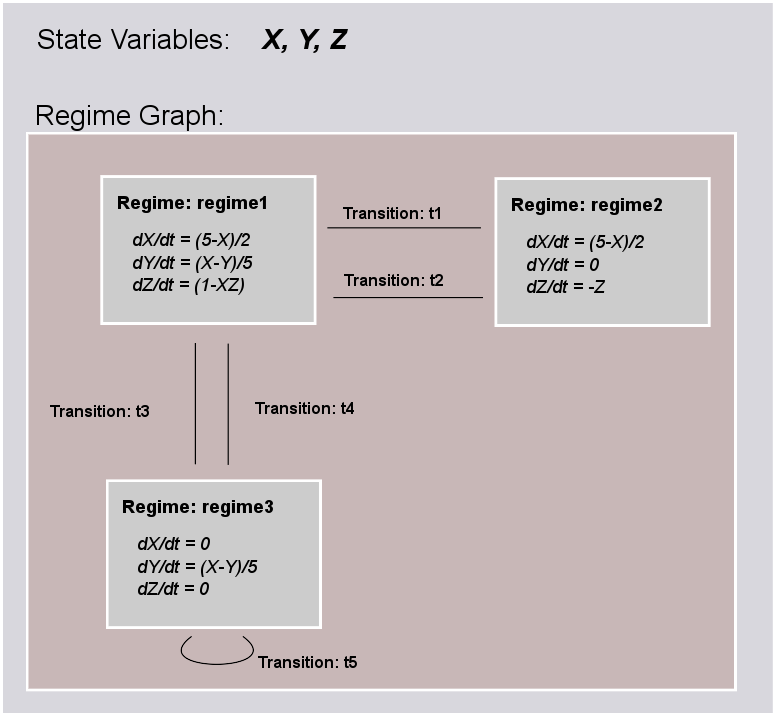
\includegraphics[width=14cm]{images/SimpleRegimeGraph.png}
\protect\caption{The dynamics block for an example component.}
\label{fig:simple_regime_graph}
\end{figure}

\subsection{Dynamics}
\label{sec:Dynamics}

\begin{table}[H]
  \begin{edtable}{tabular}{llr}
    \toprule
    \multicolumn{3}{c}{\parbox{0.55\linewidth}{\center\textbf{Dynamics Structure}}}\\
    \toprule
    \em{Element type} & \em{Multiplicity} & \em{Required} \\
    \midrule
    \StateVariable & set & no \\ 
    \Regime & set & yes\\
    \Alias & set & no\\
    \PhysicalConstant & set & no\\    
    \bottomrule
  \end{edtable}
\end{table}


The \Dynamics block represents the \emph{internal} mechanisms
governing the behaviour of the component. These dynamics are based on ordinary differential equations (ODE) but may contain non-linear transitions between
different ODE regimes. The regime graph (e.g. \ref{fig:simple_regime_graph}) must contain at least one \Regime element, and contain no regime islands. At any given time, a component will be in a single regime, and can change which regime it is in through transitions.

\note{\Alias objects are defined in Dynamics blocks, \emph{not} \Regime blocks. This means that aliases are the same across all regimes.}


\subsection{StateVariable}
\label{sec:StateVariable}

\begin{table}[H]
  \begin{edtable}{tabular}{llr}
    \toprule
    \multicolumn{3}{c}{\parbox{0.55\linewidth}{\center\textbf{StateVariable Structure}}}\\
    \toprule
    \em{Attribute name} & \em{Type/Format} & \em{Required} \\
    \midrule
    name & \identifier & yes\\
    dimension & \Dimension{}@name & yes\\
    \bottomrule
  \end{edtable}
\end{table}

The internal state of a component is defined by a set of state variables
 -- variables that can change either continuously or discontinuously as a
function of time.

The value of a \StateVariable can change in two ways:
\begin{quote}
\begin{itemize}
\item continuously through \TimeDerivative elements (in {\Regime} elements),
which define how the {\StateVariable} evolves over time, e.g.
$dX/dt=1-X$.
\item discretely through \StateAssignment (in \OnCondition or \OnEvent transition elements),
which make discrete changes to a \StateVariable value, e.g. $X = X + 1$.
\end{itemize}
\end{quote}

\subsubsection{Name attribute}
Each \StateVariable requires a \textit{name} attribute, which is a valid \identifier and uniquely identifies the \StateVariable from all other elements in the \ComponentClass.

\subsubsection{Dimension attribute}
Each \StateVariable requires a \textit{dimension} attribute. This attribute specifies the dimension of the units of the quantities that \StateVariable is expected to be initialised and updated with and should refer to the name of a \Dimension element in the global scope.


\subsection{Regime}
\label{sec:Regime}

\begin{table}[H]
  \begin{edtable}{tabular}{llr}
    \toprule
    \multicolumn{3}{c}{\parbox{0.55\linewidth}{\center\textbf{Regime Structure}}}\\
    \toprule
    \em{Attribute name} & \em{Type/Format} & \em{Required} \\
    \midrule
    name & \identifier & yes\\
    \midrule
    \em{Element type} & \em{Multiplicity} & \em{Required} \\
    \midrule
    \TimeDerivative & set & no \\ 
    \OnCondition & set & no\\
    \OnEvent & set & no\\
    \bottomrule
  \end{edtable}
\end{table}

A \Regime element represents a system of ODEs in time
on \StateVariable.  As such, \Regime defines how the state variables
change (propagate in time) between subsequent transitions. \Regime is
must have non-vanishing temporal extent. Once construction of
the \Regime is complete, it should have defined the following
properties:

\subsubsection{Name attribute}
Each \Regime requires a \textit{name} attribute, which is a valid \identifier and uniquely identifies the \Regime from all other elements in the \ComponentClass.


\subsection{TimeDerivative}
\label{sec:TimeDerivative}

\begin{table}[H]
  \begin{edtable}{tabular}{llr}
    \toprule
    \multicolumn{3}{c}{\parbox{0.55\linewidth}{\center\textbf{TimeDerivative Structure}}}\\
    \toprule
    \em{Attribute name} & \em{Type/Format} & \em{Required} \\
    \midrule
    variable & \StateVariable{}@name & yes\\
    \midrule
    \em{Element type} & \em{Multiplicity} & \em{Required} \\
    \midrule
    \MathInline & singleton & yes \\ 
    \bottomrule
  \end{edtable}
\end{table}

\TimeDerivative elements contain a mathematical expression for the right-hand side of the ODE
\begin{equation}
\frac{\mathrm{d} variable}{\mathrm{d} t} = expression
\end{equation}
which can contain of references to any combination of \StateVariable, \Parameter, \AnalogReceivePort, \AnalogReducePort and \Alias elements with the exception of aliases that are derived from \RandomDistribution components. Therefore, only one \TimeDerivative element is allowed per \StateVariable per \Regime. If a {\TimeDerivative} for a \StateVariable is not defined in a \Regime, it is assumed to be zero.

\subsubsection{Variable attribute}
Each \TimeDerivative requires a \textit{variable} attribute. This should refer to the name of a \StateVariable in the \ComponentClass. Only one \TimeDerivative is allowed per \textit{variable} in each \Regime.


\section{Transitions}
\label{sec:Transition}

Movements between dynamic regimes occurs via transitions, and have vanishing temporal extents (i.e. they are event-like). There are two types of transitions, condition-triggered transitions (see \OnCondition), which are evoked when an associated trigger expression becomes true, or event-triggered transitions (see \OnEvent), which are evoked when an associated event port receives an event from an external component.

\draftnote{Should \OnEvent transitions be able to emit new events or would this be unnecessarily complex to handle?}
During either type of transition three instantaneous actions will/can occur:
\begin{itemize}
\item The component transitions to a target regime (can be the same as the current regime)
\item State variables can be assigned new values (see \StateAssignment)
\item The component can send events (see \EventOut).
\end{itemize}

Multiple state assignments can be sent and multiple events can be sent within a single transition block
(for more on the resolution of transitions see Appendix~\ref{resolution}).

\subsection{OnCondition}
\label{sec:OnCondition}

\begin{table}[H]
  \begin{edtable}{tabular}{llr}
    \toprule
    \multicolumn{3}{c}{\parbox{0.55\linewidth}{\center\textbf{OnCondition Structure}}}\\
    \toprule
    \em{Attribute name} & \em{Type/Format} & \em{Required} \\
    \midrule
    targetRegime & \Regime{}@name & no \\
    \midrule
    \em{Element type} & \em{Multiplicity} & \em{Required} \\
    \midrule
    \Trigger & singleton & yes \\
    \StateAssignment & set & no\\
    \EventOut & set & no\\
    \bottomrule
  \end{edtable}
\end{table}

\OnCondition blocks are activated when the mathematical expression in the \Trigger block becomes true. They are typically used to model spikes in spiking neuron models, potentially emitting spike events and/or transitioning to an explicit refractory regime.

\subsubsection{TargetRegime attribute}
An \OnEvent can have a \textit{targetRegime} attribute, which should refer to the name of a \Regime element in the \ComponentClass that the dynamics block will transition to when the trigger condition is met.  If the \textit{targetRegime} attribute is omitted the regime will transition to itself.


\subsection{OnEvent}
\label{sec:OnEvent}

\vspace*{-0.25ex}
\begin{table}[H]
  \begin{edtable}{tabular}{llr}
    \toprule
    \multicolumn{3}{c}{\parbox{0.55\linewidth}{\center\textbf{OnEvent Structure}}}\\
    \toprule
    \em{Attribute name} & \em{Type/Format} & \em{Required} \\
    \midrule
    targetRegime & \Regime{}@name & no \\    
    port & \EventReceivePort{}@name & yes\\
    \midrule
    \em{Element type} & \em{Multiplicity} & \em{Required} \\
    \midrule   
    \StateAssignment & set & no\\
    \EventOut & set & no\\
    \bottomrule
  \end{edtable}
\end{table}

\OnEvent blocks are activated when the dynamics component receives an event from an external component on the port the \OnEvent element is ``listening'' to. They are typically used to model the transient response to spike events from incoming synaptic connections.

\subsubsection{Port attribute}
Each \OnEvent requires a \textit{port} attribute. This should refer to the name of an \EventReceivePort  in the \ComponentClass interface.

\subsubsection{TargetRegime attribute}
\OnEvent can have a \textit{targetRegime} attribute, which should refer to the name of a \Regime element in the \ComponentClass that the dynamics block will transition to when the \OnEvent block is triggered by an incoming event. If the \textit{targetRegime} attribute is omitted the regime will transition to itself.

\subsection{Trigger}
\label{sec:Trigger}

\begin{table}[H]
  \begin{edtable}{tabular}{llr}
    \toprule
    \multicolumn{3}{c}{\parbox{0.55\linewidth}{\center\textbf{Trigger Structure}}}\\
    \toprule
    \em{Element type} & \em{Multiplicity} & \em{Required} \\
    \midrule
    \MathInline & singleton & yes \\ 
    \bottomrule
  \end{edtable}
\end{table}

{\Trigger}s define when an {\OnCondition} transition should be occur. The \MathInline block of a
{\Trigger} can contain any arbitrary combination of `and', `or' and `negation' \emph{logical
operations} (`$\&\&$', `$||$' and `$!$' respectively) on the
result of pure inequality \emph{relational operations} (`$>$' and `$<$').
The inequality expression may contain references to 
\StateVariable, \AnalogReceivePort, \AnalogReducePort, \Parameter and {\Alias} elements, with the exception of {\Alias} elements
derived from random distributions. The \OnCondition block is triggered when the boolean result of the \Trigger statement changes from false to true. 

\subsection{StateAssignment}
\label{sec:StateAssignment}

\begin{table}[H]
  \begin{edtable}{tabular}{llr}
    \toprule
    \multicolumn{3}{c}{\parbox{0.55\linewidth}{\center\textbf{StateAssignment Structure}}}\\
    \toprule
    \em{Attribute name} & \em{Type/Format} & \em{Required} \\
    \midrule
    variable & \StateVariable{}@name & yes\\
    \midrule
    \em{Element type} & \em{Multiplicity} & \em{Required} \\
    \midrule
    \MathInline & singleton & yes \\     
    \bottomrule
  \end{edtable}
\end{table}

\StateAssignment elements allow discontinuous changes in the value of state variables. Only one state assignment is allowed per variable per transition block. The assignment expression may contain references to 
\StateVariable, \AnalogReceivePort, \AnalogReducePort, \Parameter and {\Alias} elements, including {\Alias}
elements derived from random distributions. State assignments are typically used to reset the membrane voltage after an outgoing spike event or update post-synaptic response states after an incoming spike event.

\subsubsection{Variable attribute}
Each \StateAssignment requires a \textit{variable} attribute. This should refer to the name of a \StateVariable in the \ComponentClass. Only one \StateAssignment is allow per \textit{variable} in each \OnEvent or \OnCondition block.

\subsection{EventOut}
\label{sec:EventOut}

\begin{table}[H]
  \begin{edtable}{tabular}{llr}
    \toprule
    \multicolumn{3}{c}{\parbox{0.55\linewidth}{\center\textbf{EventOut Structure}}}\\
    \toprule
    \em{Attribute name} & \em{Type/Format} & \em{Required} \\
    \midrule
    port & \EventSendPort{}@name & yes\\
    \bottomrule
  \end{edtable}
\end{table}

\EventOut elements specify events to be raised during a transition. They are typically used to raise spike events from within \OnCondition elements.

\subsubsection{Port attribute}
Each \EventOut requires a \textit{port} attribute. This should refer to the name of an \EventSendPort in the \ComponentClass interface.

\section{Random Distributions}

\subsection{RandomDistribution}
\label{sec:RandomDistribution}

\begin{table}[H]
  \begin{edtable}{tabular}{llr}
    \toprule
    \multicolumn{3}{c}{\parbox{0.55\linewidth}{\center\textbf{RandomDistribution Structure}}}\\
    \toprule
    \em{Attribute name} & \em{Type/Format} & \em{Required} \\
    \midrule
    standardLibrary & \URL & yes\\
    \bottomrule
  \end{edtable}
\end{table}

As of version 1.0, the only random distributions available to the user are those defined in the standard library. The names and parameters of the random distribution in the standard library match the UncertML definitions that can be found at \href{http://www.uncertml.org/distributions}{http://www.uncertml.org/distributions}. The subset of the UncertML distributions that should be implemented are by NineML compliant packages are,

\begin{itemize}
\item BernoulliDistribution
\item BetaDistribution
\item BinomialDistribution
\item CauchyDistribution
\item ChiSquareDistribution
\item DirichletDistribution
\item ExponentialDistribution
\item FDistribution
\item GammaDistribution
\item GeometricDistribution
\item HypergeometricDistribution
\item InverseGammaDistribution
\item LaplaceDistribution
\item LogisticDistribution
\item LogNormalDistribution
\item MixtureModel
\item MultinomialDistribution
\item NegativeBinomialDistribution
\item NormalDistribution
\item NormalInverseGammaDistribution
\item ParetoDistribution
\item PoissonDistribution
\item StudentTDistribution
\item UniformDistribution
\item WeibullDistribution
\end{itemize}

~

\note{\textit{C} implementations of these distributions are available in the GNU Scientific Library, \href{http://www.gnu.org/software/gsl/}{http://www.gnu.org/software/gsl/}}

\subsubsection{StandardLibrary attribute}
The \textit{standardLibrary} attribute is required and should point to a \URL in the \href{http://www.uncertml.org/distributions/}{http://www.uncertml.org/distributions/} directory.


\section{Network Connectivity}

\subsection{ConnectionRule}
\label{sec:ConnectionRule}

\begin{table}[H]
  \begin{edtable}{tabular}{llr}
    \toprule
    \multicolumn{3}{c}{\parbox{0.55\linewidth}{\center\textbf{ConnectionRule Structure}}}\\
    \toprule
    \em{Attribute name} & \em{Type/Format} & \em{Required} \\
    \midrule
    standardLibrary & \URL & yes\\
    \bottomrule
  \end{edtable}
\end{table}

In Version 1.0 of the NineML standard, connection rules must be one of 6 standard library types (in future versions, built-in connectivity rules are to be replaced with arbitrary connection rule generators):
\begin{itemize}
\item AllToAll
\item OneToOne
\item ProbabilisticConnectivity
\item ExplicityConnectionList
\item RandomFanOut
\item RandomFanIn
\end{itemize}

\subsubsection{StandardLibrary attribute}
The \textit{standardLibrary} attribute is required and should point to a \URL in the \href{http://nineml.net/standardlibraries/connectionrules/}{http://nineml.net/standardlibraries/connectionrules/} directory.

\emph{\textbf{http://nineml.net/standardlibraries/connectionrules/AllToAll}}

All cells in the source population are connected to all cells in the destination population.

\emph{\textbf{http://nineml.net/standardlibraries/connectionrules/OneToOne}}

Each cell in the source population is connected to the cell in the destination population with the corresponding index. Note that this requires that the source and destination populations be the same size.

\emph{\textbf{http://nineml.net/standardlibraries/connectionrules/ProbabilisticConnectivity}}

All cells in the source population are connected to cells in the destination population with a probability defined by a parameter, which should be named \textit{probability}. The properties supplied to the \textit{probability} parameter should either be a \SingleValue representing the probability of a connection between all source and destination cell pairs, or a \ArrayValue or \ExternalArrayValue of size $M{\times}N$, where $M$ and $N$ are the size of the source and destination populations respectively. In the case of the \ArrayValue or \ExternalArrayValue properties, the list represents probabilities of connections existing between the first cell in the source population with every cell in the destination population in order of their index, followed by the second cell in the source with with every cell in the destination population in order of their index and so forth for each cell in the source population.

\emph{\textbf{http://nineml.net/standardlibraries/connectionrules/ExplicitConnectionList}}

Cells in the source population are connected to cells in the destination population as specified by an explicit arrays. The source and destination are defined via parameters, which should be named \textit{sourceIndicies} and \textit{destinationIndicies} parameters respectively.

The properties supplied to the \textit{sourceIndicies} parameter should be a \ArrayValue or \ExternalArrayValue drawn from the set $\{1,\ldots,M\}$ where $M$ is the size of the source population and be the same length as the property supplied to the \textit{target-indices} parameter.

The properties supplied to the \textit{destinationIndicies} parameter should be a \ArrayValue or \ExternalArrayValue drawn from the set $\{1,\ldots,N\}$ where $N$ is the size of the source population and be the same length as the property supplied to the \textit{source-indices} parameter.

\emph{\textbf{http://nineml.net/standardlibraries/connectionrules/RandomFanOut}}

Cells in the source population are connected to cells in the destination population with a probability defined by a parameter, which should be named \textit{probability}. The property supplied to the \textit{probability} parameter should be a \SingleValue.

\emph{\textbf{http://nineml.net/standardlibraries/connectionrules/RandomFanIn}}

Cells in the destination population are connected to cells in the source population with a probability defined by a parameter, which should be named \textit{probability}. The property supplied to the \textit{probability} parameter should be a \SingleValue.

\clearpage
\part{User Layer}
\section{Components and Properties}

\subsection{Component}
\label{sec:Component}

\begin{table}[H]
  \begin{edtable}{tabular}{llr}
    \toprule
    \multicolumn{3}{c}{\parbox{0.55\linewidth}{\center\textbf{Component Structure}}}\\
    \toprule
    \em{Attribute name} & \em{Type/Format} & \em{Required} \\
    \midrule
    name & \identifier & yes\\
    \midrule
    \em{Element type} & \em{Multiplicity} & \em{Required} \\
    \midrule
    \Definition | \Prototype & singleton & yes \\ 
    \Property & set & no\\
    \bottomrule
  \end{edtable}
\end{table}

\Component elements instantiate Abstraction Layer component classes by providing properties 
for each of the parameters defined the class. Each \Component is linked to a \ComponentClass
class by a \Definition element, which locates the component class. A \Component 
that instantiates a \ComponentClass directly must supply matching \Property elements for each \Parameter in the \ComponentClass. Alternatively, a \Component can inherit a \ComponentClass and set of \Property elements from an existing component by substituting the \Definition for a \Prototype element, which locates the reference \Component. In this case, only the properties that differ from the reference component need to be specified.

\subsubsection{Name attribute}
Each \Component requires a \textit{name} attribute, which should be a valid \identifier and uniquely identify the {\Component} from all other elements in the global scope.

\subsection{Definition}
\label{sec:Definition}

\begin{table}[H]
  \begin{edtable}{tabular}{llr}
    \toprule
    \multicolumn{3}{c}{\parbox{0.55\linewidth}{\center\textbf{Definition Structure}}}\\
    \toprule
    \em{Attribute name} & \em{Type/Format} & \em{Required} \\
    \midrule
    url & \URL & no\\
    \midrule
    \em{Text format} & \; & \em{Required} \\
    \midrule
    \ComponentClass{}@name & \; & yes \\ 
    \bottomrule
  \end{edtable}
\end{table}

The \Definition element establishes a link between a User Layer component and Abstraction Layer
\ComponentClass. This \ComponentClass can be located either in the current
document or in another file if a \textit{url} attribute is provided.

\subsubsection{Url attribute}
If the \ComponentClass referenced by the definition element is defined outside the current document, the \textit{url} attribute specifies a \URL for the file which contains the \ComponentClass definition. If it is omitted the \ComponentClass is assumed to be in the current document.

\subsubsection{Text format}
The name of the \ComponentClass to be referenced \ComponentClass needs to be provided in the text of \Definition element.

\subsection{Prototype}
\label{sec:Prototype}

\begin{table}[H]
  \begin{edtable}{tabular}{llr}
    \toprule
    \multicolumn{3}{c}{\parbox{0.55\linewidth}{\center\textbf{Prototype Structure}}}\\
    \toprule
    \em{Attribute name} & \em{Type/Format} & \em{Required} \\
    \midrule
    url & \href{http://en.wikipedia.org/wiki/Uniform_resource_locator}{URL} & no\\
    \midrule
    \em{Text format} & \; & \em{Required} \\
    \midrule
    \Component{}@name & \; & yes \\ 
    \bottomrule
  \end{edtable}
\end{table}

The \Prototype element establishes a link to an existing User Layer \Component, which defines the \ComponentClass and default properties of the \Component.  The reference \Component can be located either in the current
document or in another file if a \textit{url} attribute is provided.

\subsubsection{Url attribute}
If the prototype \Component is defined outside the current file, the \textit{URL} attribute specifies a \URL for the file which contains the prototype \Component.

\subsubsection{Text format}
The name of the \Component to be referenced \Component needs to be provided in the text of \Prototype element.

\draftnote{I have removed the \Quantity{s} in favour of adding units to the \Property elements as it seemed superfluous and incongruous with the AL (i.e. \Parameter s define the dimension). I will create a GitHub issue about this where we can discuss this and potentially decide to change it back if you like}
\subsection{Property}
\label{sec:Property}

\begin{table}[H]
  \begin{edtable}{tabular}{llr}
    \toprule
    \multicolumn{3}{c}{\parbox{0.55\linewidth}{\center\textbf{Property Structure}}}\\
    \toprule
    \em{Attribute name} & \em{Type/Format} & \em{Required} \\
    \midrule
    name & \Parameter{}@name & yes\\
    units & \Unit{}@symbol & yes\\
    \midrule
    \em{Element type} & \em{Multiplicity} & \em{Required} \\
    \midrule
    \SingleValue | \ArrayValue | \ExternalArrayValue | \ComponentValue & singleton & yes \\ 
    \bottomrule
  \end{edtable}
\end{table}

\Property elements provide values for the parameters defined in the \ComponentClass
of the \Component. Their \textit{name} attribute should match the name of the corresponding \Parameter element in the \ComponentClass. The \Property should be provided units that match the dimensionality of the corresponding \Parameter definition.

\subsubsection{Name attribute}
Each \Property requires a \textit{name} attribute. This should refer to the name of a \Parameter in the corresponding \ComponentClass of the \Component.

\subsubsection{Units attribute}
Each \Property element requires a \emph{units} attribute. The \textit{units} attribute specifies the units of the quantity and should refer to the name of a \Unit element in the global scope. For a dimensionless units a \Unit\withelem\Dimension with no SI dimensions can be used. The SI dimensions of the \Unit\withelem\Dimension should match the SI dimensions of the corresponding \Parameter\withelem\Dimension.

\subsection{Reference}
\label{sec:Reference}

\begin{table}[H]
  \begin{edtable}{tabular}{llr}
    \toprule
    \multicolumn{3}{c}{\parbox{0.55\linewidth}{\center\textbf{Reference Structure}}}\\
    \toprule
    \em{Attribute name} & \em{Type/Format} & \em{Required} \\
    \midrule
    url &  \href{http://en.wikipedia.org/wiki/Uniform_resource_locator}{URL}  & no\\
    \midrule
    \em{Text format} & \; & \em{Required} \\
    \midrule
    *@name & \; & yes\\
    \bottomrule
  \end{edtable}
\end{table}

\Reference elements are used to locate User Layer elements in the global scope of the current separate documents. In most cases, User Layer elements (with the exception of \Population elements supplied to \Projection) can be specified inline, i.e. within the element they are required. However, it is often convenient to define a component in the global scope as this allows it to be reused at different places within the model. The \textit{url} attribute can be used to reference a component in a separate document, potentially one published online in a public repository (e.g. \href{http://senselab.med.yale.edu/modeldb/ListByModelName.asp?c=19&lin=-1}{ModelDB} or \href{http://www.opensourcebrain.org/}{Open Source Brain}).

\subsubsection{Url attribute}
The \textit{url} attribute specifies a \URL for the file which contains the User Layer element to be referenced.

\subsubsection{Text format}
The name of the User Layer element to be referenced should be included in the text of the \Reference element.

\section{Values}
\label{sec:Values}

In NineML, ``values'' are arrays that implicitly grow to fill the size of the container (i.e. \Population or \Projection) they are located within. Values can be one of four types
\begin{itemize}
\item \SingleValue, a consistent value across the container
\item \ArrayValue, an explicit array defined in NineML
\item \ExternalArrayValue, an explicit array defined in text (space delimited) or HDF5 format.
\item \ComponentValue, a return value from a \RandomDistribution component.
\end{itemize}

\subsection{SingleValue}
\label{sec:SingleValue}

\begin{table}[H]
  \begin{edtable}{tabular}{llr}
    \toprule
    \multicolumn{3}{c}{\parbox{0.55\linewidth}{\center\textbf{SingleValue Structure}}}\\
    \toprule
    \em{Text format} & \; & \em{Required} \\
    \midrule
    \primtype{real number} & \; & yes \\ 
    \bottomrule
  \end{edtable}
\end{table}

A \SingleValue element represents an array filled with a single value.

\subsubsection{Text format}
Any valid numeric value in \href{http://en.wikipedia.org/wiki/ANSI_C}{ANSI C89}, including shorthand scientific notation  e.g. 1e-5 ($1\times10^{-5}$).

\subsection{ArrayValue}
\label{sec:ArrayValue}

\begin{table}[H]
  \begin{edtable}{tabular}{llr}
    \toprule
    \multicolumn{3}{c}{\parbox{0.55\linewidth}{\center\textbf{ArrayValue Structure}}}\\
    \toprule
    \em{Element type} & \em{Multiplicity} & \em{Required} \\
    \midrule
    \ArrayValueRow & set & no \\
    \bottomrule
  \end{edtable}
\end{table}

\ArrayValue elements are used to represent an explicit array of values in XML. \ArrayValue elements contain a set of \ArrayValueRow elements (i.e. unordered, since they are explicitly ordered by their \textit{index} attribute). Since XML is significantly slower to parse than plain text and binary formats it is not recommended to use \ArrayValue for large arrays, preferring \ExternalArrayValue instead. 

\subsection{ArrayValueRow}
\label{sec:ArrayValueRow}

\begin{table}[H]
  \begin{edtable}{tabular}{llr}
    \toprule
    \multicolumn{3}{c}{\parbox{0.55\linewidth}{\center\textbf{ArrayValueRow Structure}}}\\
    \toprule
    \em{Attribute name} & \em{Type/Format} & \em{Required} \\
    \midrule
    index & integer & yes \\
    \midrule
    \em{Text format} & \; & \em{Required} \\
    \midrule
    \primtype{real number} & \; & yes\\
    \bottomrule
  \end{edtable}
\end{table}

\ArrayValueRow elements represent the numerical values of the explicit \ArrayValue element.
\subsubsection{Index attribute}
The \textit{index} attribute specifies the index of the \ArrayValueRow in the \ArrayValue. It must be non-negative, unique amongst the set of \ArrayValueRow{}@index in the list, and the set of indices must be contiguous for a single \ArrayValue.

\note{The order of {\ArrayValueRow} elements within an \ArrayValue element does not effect the interpreted order of the values in the array in keeping with the order non-specific design philosophy of NineML (see \ref{sec:design_considerations}).}

\subsubsection{Text format}
Any valid numeric value in \href{http://en.wikipedia.org/wiki/ANSI_C}{ANSI C89}, including shorthand scientific notation  e.g. 1e-5 ($1\times10^{-5}$).

\subsection{ExternalArrayValue}
\label{sec:ExternalArrayValue}

\begin{table}[H]
  \begin{edtable}{tabular}{llr}
    \toprule
    \multicolumn{3}{c}{\parbox{0.55\linewidth}{\center\textbf{ExternalArrayValue Structure}}}\\
    \toprule
    \em{Attribute name} & \em{Type/Format} & \em{Required} \\
    \midrule
    url & \href{http://en.wikipedia.org/wiki/Uniform_resource_locator}{URL} & yes\\
    mimeType & \href{http://en.wikipedia.org/wiki/Internet_media_type}{MIME type}  & yes\\
    columnName & Data column name in external file & yes\\    
    \bottomrule
  \end{edtable}
\end{table}

\ExternalArrayValue elements are used to explicitly define large arrays of values. The array data are not stored in XML (which is slow to parse) but more efficient text or binary \href{http://www.hdfgroup.org/HDF5/}{HDF5 (http://www.hdfgroup.org/HDF5/)} formats. As of version 1.0, the data in the external files are stored as dense \primtype{float} or \primtype{integer} arrays. However, sparse-array formats are planned for future versions.

The \textit{columnName} attribute of the \ExternalArrayValue elements allows multiple arrays of equal length (and therefore typically relating to the same container) to be stored in the same external file. 

\subsubsection{Url attribute}
The \textit{url} attribute specifies the \URL of the external data file.

\subsubsection{MimeType attribute}
The \textit{mimetype} attribute specifies the data format for the external value list in the \href{http://en.wikipedia.org/wiki/Internet_media_type}{MIME type} syntax. Currently, only two formats are supported \lstinline|application/vnd.nineml.valuelist.text| and \lstinline|application/vnd.nineml.valuelist.hdf5|. 

\begin{itemize}
\item \lstinline|application/vnd.nineml.externalvaluearray.text| - an ASCII text file with a single row of white-space separated column names, followed by arbitrarily many white-space separated data rows of numeric values. Each numeric value is associated with the column name corresponding to the same index the along the row. Therefore, the number of items in each row must be the same.
\item \lstinline|application/vnd.nineml.externalvaluearray.hdf5| - a \href{http://www.hdfgroup.org/HDF5/}{HDF5} data file containing a single level of named members of \primtype{array->float} or \primtype{array->int} type.
\end{itemize}

\subsubsection{ColumnName attribute}

Each \ExternalArrayValue must have a \textit{columnName} attribute, which refers to a column header in the external data file. 

\draftnote{What do you think of this? This allows a single component to return two (related) values at different places at the model (e.g. weight and delay in distance dependent rules). It also seemed a bit neater}
\subsection{ComponentValue}
\label{sec:ComponentValue}

\begin{table}[H]
  \begin{edtable}{tabular}{llr}
    \toprule
    \multicolumn{3}{c}{\parbox{0.55\linewidth}{\center\textbf{ExternalArrayValue Structure}}}\\
    \toprule
    \em{Attribute name} & \em{Type/Format} & \em{Required} \\
    \midrule
    port & {\AnalogSendPort}@name & yes\\
    \midrule    
    \em{Element type} & \em{Multiplicity} & \em{Required} \\
    \midrule
    \Component{}\withelem\RandomDistribution | \Reference{}\pointto\Component{}\withelem\RandomDistribution & singleton & yes \\
    \bottomrule
  \end{edtable}
\end{table}

The array of values represented by a \ComponentValue element is populated from the output port of a component. As of version 1.0, only \RandomDistribution components are supported within \ComponentValue but function and generator components are planned for later versions. The size of the generated array is determined by the size of the container (i.e. \Population or \Projection) the \ComponentValue is nested within.

\subsubsection{Port attribute}
Each \ComponentValue requires a \textit{port} attribute, which selects which port of the \Component to read.

\section{Populations}

\subsection{Population}
\label{sec:Population}

\begin{table}[H]
  \begin{edtable}{tabular}{llr}
    \toprule
    \multicolumn{3}{c}{\parbox{0.55\linewidth}{\center\textbf{Population Structure}}}\\
    \toprule
    \em{Attribute name} & \em{Type/Format} & \em{Required} \\
    \midrule
    name & \identifier & yes\\
    \midrule
    \em{Element type} & \em{Multiplicity} & \em{Required} \\
    \midrule
    \Number & singleton & yes \\
    \Cell & singleton & yes \\
    \bottomrule
  \end{edtable}
\end{table}

A \Population defines a set of dynamic components of the same class. The size of the set is specified by the \Number element. The properties of the dynamic components are generated from value types, which can be constant across the population, randomly distributed or individually specified (see \ref{sec:Values}).

\subsubsection{Name attribute}
Each \Population requires a \textit{name} attribute, which should be a valid \identifier and uniquely identify the {\Population} from all other elements in the global scope.

\subsection{Cell}
\label{sec:Cell}

\begin{table}[H]
  \begin{edtable}{tabular}{llr}
    \toprule
    \multicolumn{3}{c}{\parbox{0.55\linewidth}{\center\textbf{Cell Structure}}}\\
    \toprule
    \em{Element type} & \em{Multiplicity} & \em{Required} \\
    \midrule
    \Component{}\withelem\Dynamics | \Reference{}\pointto\Component{}\withelem\Dynamics & singleton & yes \\
    \bottomrule
  \end{edtable}
\end{table}

The \Cell element specifies the dynamic components that will make up the population. The \Component can be defined inline or via a \Reference element. 

\subsection{Number}
\label{sec:Number}

\begin{table}[H]
  \begin{edtable}{tabular}{llr}
    \toprule
    \multicolumn{3}{c}{\parbox{0.55\linewidth}{\center\textbf{Number Structure}}}\\
    \toprule
    \em{Text format} & \; & \em{Required} \\
    \midrule
    \primtype{integer} & \; & yes\\
    \bottomrule
  \end{edtable}
\end{table}

The number of cells in the population is specified by the integer provided in the text of the \Number element. In future versions this may be extended to allow the size of a population to be derived from other features of the \Population. 

\subsubsection{Text format}
The text of the \Number element contains an \primtype{integer} representing the size of the population.

\section{Projections}

Projections define the synaptic connectivity between two populations, the post-synaptic response of the connections, the plasticity rules that modulate the post-synaptic response and the transmission delays. Synaptic and plasticity dynamic components are created and connected to and from explicitly defined ports of the cell components in the source and projection populations if the connection rule determines there is a connection between a particular source and destination cell pair. 

\SingleValue and \ComponentValue elements used in properties of a projection (in the \Connectivity and \Synapse elements) take the size of the number of connections made. While \ArrayValue and \ExternalArrayValue elements can either be the size of the number of connections made or the number of possible unique connections (i.e. $N_{\mathrm{source}} * N_{\mathrm{dest}}$). In either case, the expected array data is ordered by the indices
\begin{equation}
i_{\mathrm{value}} = i_{\mathrm{source}} * N_{\mathrm{dest}} + i_{\mathrm{dest}}
\end{equation}
where $i_{\mathrm{value}}$, $i_{\mathrm{source}}$ and $i_{\mathrm{dest}}$ are the indices of the array entry, and the source and destination cells respectively (starting from 0), and $N_{\mathrm{dest}}$ is the size of the destination population. For the case of the explicit arrays being the size of the number connections made, data for $i_{\mathrm{value}}$ indices that do not correspond to connected pairs are omitted.

\subsection{Projection}
\label{sec:Projection}

\begin{table}[H]
  \begin{edtable}{tabular}{llr}
    \toprule
    \multicolumn{3}{c}{\parbox{0.55\linewidth}{\center\textbf{Projection Structure}}}\\
    \toprule
    \em{Attribute name} & \em{Type/Format} & \em{Required} \\
    \midrule
    name & \identifier & yes\\
    \midrule
    \em{Element type} & \em{Multiplicity} & \em{Required} \\
    \midrule
    \Source & singleton & yes \\ 
    \Destination & singleton & yes \\
    \Connectivity & singleton & yes \\
    \Synapse & singleton & yes \\
    \bottomrule
  \end{edtable}
\end{table}

The \Projection element contains all the elements that define a projection between two populations and should be uniquely identified in the scope of the document.

\subsubsection{Name attribute}
Each \Projection requires a \textit{name} attribute, which should be a valid \identifier and uniquely identify the {\Projection} from all other elements in the global scope.


\subsection{Connectivity}
\label{sec:Connectivity}

\begin{table}[H]
  \begin{edtable}{tabular}{llr}
    \toprule
    \multicolumn{3}{c}{\parbox{0.55\linewidth}{\center\textbf{Connectivity Structure}}}\\
    \toprule
    \em{Element type} & \em{Multiplicity} & \em{Required} \\
    \midrule
    \Component{}\withelem\ConnectionRule & singleton & yes \\ 
    \bottomrule
  \end{edtable}
\end{table}

The \Connectivity element contains a \Component\withelem\ConnectionRule, which defines how the source and destination populations are connected together. 

\subsection{Source}
\label{sec:Source}

\begin{table}[H]
  \begin{edtable}{tabular}{llr}
    \toprule
    \multicolumn{3}{c}{\parbox{0.55\linewidth}{\center\textbf{Source Structure}}}\\
    \toprule
    \em{Element type} & \em{Multiplicity} & \em{Required} \\
    \midrule
    \Reference{}\pointto\Population | \Reference{}\pointto\Selection & singleton & yes \\
    \ReceiveConnection & set & no\\
    \bottomrule
  \end{edtable}
\end{table}

The \Source element specifies the pre-synaptic population or selection (see \Selection) of the projection and all the port connections it receives. The source population is specified via a \Reference element since it should not be defined within the \Projection. The source population can receive incoming port connections from the \Synapse element (see \FromSynapse). Connections with these ports are only made if the \Connectivity\withelem\ConnectionRule determines that the source and destination cells should be connected.

\subsection{Destination}
\label{sec:Destination}

\begin{table}[H]
  \begin{edtable}{tabular}{llr}
    \toprule
    \multicolumn{3}{c}{\parbox{0.55\linewidth}{\center\textbf{Destination Structure}}}\\
    \toprule
    \em{Element type} & \em{Multiplicity} & \em{Required} \\
    \midrule
    \Reference{}\pointto\Population | \Reference{}\pointto\Selection & singleton & yes \\
    \ReceiveConnection & set & yes\\
    \bottomrule
  \end{edtable}
\end{table}

The \Destination element specifies the post-synaptic or selection (see \Selection) population of the projection and all the port connections it receives. The destination population is specified via a \Reference element since it should not be defined within the \Projection. The source population can receive incoming port connections from the the \Synapse element (see \FromSynapse). Connections with these ports are only made if the \Connectivity\withelem\ConnectionRule determines that the source and destination cells should be connected.

\subsection{Synapse}
\label{sec:Synapse}

\begin{table}[H]
  \begin{edtable}{tabular}{llr}
    \toprule
    \multicolumn{3}{c}{\parbox{0.55\linewidth}{\center\textbf{Response Structure}}}\\
    \toprule
    \em{Element type} & \em{Multiplicity} & \em{Required} \\
    \midrule
    \Component{}\withelem\Dynamics | \Reference{}\pointto\Component{}\withelem\Dynamics & singleton & yes \\ 
    \ReceiveConnection & set & yes\\
    \bottomrule
  \end{edtable}
\end{table}

The \Synapse defines the effect on the post-synaptic cell dynamics of an incoming synaptic input. The additional dynamics are defined by a \Component\withelem\Dynamics element, which can be defined inline or referenced. For static connections the magnitude of the response (i.e. synaptic weight) is typically passed as a property of the \Synapse element.

The post-synaptic response dynamics can receive incoming port connections from either the pre or post synaptic populations (see \FromSource and \FromDestination). A \Synapse object is implicitly created and connected to these ports if the \Connectivity\withelem\ConnectionRule determines that the source and destination cells should be connected.

It is recommended to factor out plasticity rules from post-synaptic response dynamics and combine them within \MultiComponent element to promote reusability of response and plasticity dynamics. 

\subsection{ReceiveConnection}
\label{sec:ReceiveConnection}

\begin{table}[H]
  \begin{edtable}{tabular}{llr}
    \toprule
    \multicolumn{3}{c}{\parbox{0.55\linewidth}{\center\textbf{ReceiveConnection Structure}}}\\
    \toprule
    \em{Attribute name} & \em{Type/Format} & \em{Required} \\
    \midrule \relax
    port & [\EventReceivePort{} | \AnalogReceivePort{} | \AnalogReducePort{}]@name & yes\\
    \midrule \relax
    \em{Element type} & Multiplicity & \em{Required} \\
    \midrule \relax
    From* & set & yes\\
    \bottomrule
  \end{edtable}
\end{table}

The \ReceiveConnection element specifies a receive port which will receive a connection from a port on a remote component. Depending on the context where \ReceiveConnection the components it can receive from vary, hence there are various elements, all named \emph{From*}, specifying the relationship of the remote component to the enclosing element (e.g. \FromSource, \FromDestination and \FromSynapse  in \Projection containers).

\subsubsection{Port attribute}
Each \ReceiveConnection element requires a \textit{port} attribute. This should refer to the name of a \AnalogReceivePort, \EventReceivePort or \AnalogReducePort in the \ComponentClass associated with the enclosing element.

\subsection{FromSource}
\label{sec:FromSource}

\begin{table}[H]
  \begin{edtable}{tabular}{llr}
    \toprule
    \multicolumn{3}{c}{\parbox{0.55\linewidth}{\center\textbf{FromSource Structure}}}\\
    \toprule
     \em{Attribute name} & \em{Type/Format} & \em{Required} \\
    \midrule
    port & [\AnalogSendPort | \EventSendPort{}]@name & yes\\
    \midrule \relax
    \em{Element type} & Multiplicity & \em{Required} \\
    \midrule \relax
    \Delay & singleton & yes\\
    \bottomrule
  \end{edtable}
\end{table}

The \FromSource element specifies a port connection to the projection component (either the destination cell, post-synaptic response or plasticity dynamics) inside which it is inserted from the source cell dynamics.

\subsubsection{port attribute}
Each \FromSource element requires a \textit{port} attribute. This should refer to the name of a \AnalogSendPort or \EventSendPort in the \Source\withelem\Cell{}\withelem\Component{}\withelem\ComponentClass. The transmission mode of the port (i.e. \lq\lq{}analog\rq\rq{} or \lq\lq{}event\rq\rq{}) should match that of the port referenced by the enclosing \ReceiveConnection element.

\subsection{FromDestination}
\label{sec:FromDestination}

\begin{table}[H]
  \begin{edtable}{tabular}{llr}
    \toprule
    \multicolumn{3}{c}{\parbox{0.55\linewidth}{\center\textbf{FromDestination Structure}}}\\
    \toprule
     \em{Attribute name} & \em{Type/Format} & \em{Required} \\
    \midrule
    port & [\AnalogSendPort | \EventSendPort{}]@name & yes\\
    \bottomrule
  \end{edtable}
\end{table}

The \FromDestination element specifies a port connection to the projection component (either the source cell, post-synaptic response or plasticity dynamics) inside which it is inserted from the destination cell dynamics.

\subsubsection{port attribute}
Each \FromDestination element requires a \textit{port} attribute. This should refer to the name of a \AnalogSendPort or \EventSendPort in the \Destination\withelem\Cell\withelem\Component{}\withelem\ComponentClass. The transmission mode of the port (i.e. \lq\lq{}analog\rq\rq{} or \lq\lq{}event\rq\rq{}) should match that of the port referenced by the enclosing \ReceiveConnection element.


\subsection{FromSynapse}
\label{sec:FromSynapse}

\begin{table}[H]
  \begin{edtable}{tabular}{llr}
    \toprule
    \multicolumn{3}{c}{\parbox{0.55\linewidth}{\center\textbf{FromSynapse Structure}}}\\
    \toprule
     \em{Attribute name} & \em{Type/Format} & \em{Required} \\
    \midrule
    port & [\AnalogSendPort | \EventSendPort{}]@name & yes\\
    \bottomrule
  \end{edtable}
\end{table}

The \FromSynapse element specifies a port connection to the source or destination cell component from the \Synapse element.

\subsubsection{port attribute}
Each \FromSynapse element requires a \textit{port} attribute. This should refer to the name of a \AnalogSendPort or \EventSendPort in the \Synapse\withelem\ComponentClass. The transmission mode of the port (i.e. \lq\lq{}analog\rq\rq{} or \lq\lq{}event\rq\rq{}) should match that of the port referenced by the enclosing \ReceiveConnection element.

\subsection{Delay}
\label{sec:Delay}

\begin{table}[H]
  \begin{edtable}{tabular}{llr}
    \toprule
    \multicolumn{3}{c}{\parbox{0.55\linewidth}{\center\textbf{Delay Structure}}}\\
    \toprule
     \em{Attribute name} & \em{Type/Format} & \em{Required} \\
    \midrule
    units & \Unit{}@symbol & yes\\
    \midrule
    \em{Element type} & \em{Multiplicity} & \em{Required} \\
    \midrule
    \SingleValue | \ArrayValue | \ExternalArrayValue | \ComponentValue & singleton & yes \\ 
    \bottomrule
  \end{edtable}
\end{table}

In the current version, the \Delay element specifies the delay between the pre-synaptic cell port and the \Synapse. In future versions, it is planned to expand the delay architecture to allow delays on any port connections to allow finer control of the delay between the different components.

\subsubsection{Units attribute}
The \textit{units} attribute specifies the units of the delay and should refer to the name of a \Unit element in the global scope. The \Unit{}\withelem\Dimension should be temporal, i.e. have $t=1$ and all other SI dimensions set to 0. 

\section{Selections: combining populations and subsets}

Selections are designed to allow sub and super-sets of cell populations to be projected to/from other populations (or selections thereof). In version 1.0, the only supported operation is the concatenation of multiple populations into super-sets but in future versions it is planned to provide ``slicing'' operations to select sub sets of populations. 

\subsection{Selection}
\label{sec:Selection}

\begin{table}[H]
  \begin{edtable}{tabular}{llr}
    \toprule
    \multicolumn{3}{c}{\parbox{0.55\linewidth}{\center\textbf{Selection Structure}}}\\
    \toprule
    \em{Element type} & \em{Multiplicity} & \em{Required} \\
    \midrule
    \Concatenate & singleton & yes \\ 
    \bottomrule
  \end{edtable}
\end{table}

The \Selection element contains the operations that are used to select the cells to add to the selection.
\subsection{Concatenate}
\label{sec:Concatenate}

\begin{table}[H]
  \begin{edtable}{tabular}{llr}
    \toprule
    \multicolumn{3}{c}{\parbox{0.55\linewidth}{\center\textbf{Concatenate Structure}}}\\
    \toprule
    \em{Element type} & \em{Multiplicity} & \em{Required} \\
    \midrule
    \Item & set & yes \\ 
    \bottomrule
  \end{edtable}
\end{table}

The \Concatenate element is used to add populations to a selection. It contains a set of \Item elements which reference the \Population elements to be concatenated. The order of the \Item elements does not effect the order of the concatenation, which is determined by the \emph{index} attribute of the \Item elements. The indices must start from 0 and cover the range to $N-1$, where $N$ is the population size (i.e. $i=0,\ldots,N-1$).

\subsection{Item}
\label{sec:Item}

\begin{table}[H]
  \begin{edtable}{tabular}{llr}
    \toprule
    \multicolumn{3}{c}{\parbox{0.55\linewidth}{\center\textbf{Item Structure}}}\\
    \toprule
    \em{Attribute name} & \em{Type/Format} & \em{Required} \\
    \midrule
    index & \primtype{integer} & yes\\
    \midrule
    \em{Element type} & Multiplicity & \em{Required} \\
    \midrule \relax
    \Reference{}\pointto{}[\Population | \Selection{}] & singleton & yes\\
    \bottomrule
  \end{edtable}
\end{table}

Each \Item element references as a \Population or \Selection element and specifies their order in the concatenation.

\subsubsection{Index attribute}
Each \Item requires a \textit{index} attribute. This attribute specifies the order in which the {\Population}s in the \Selection are concatenated and thereby the indices of the cells within the combined \Selection. 

\note{This preserves the order non-specific nature of elements in NineML}

\clearpage
\part{Standard Extensions}

\section{Multi-component models}

Multi-component models enable component classes to be constructed out of smaller sub-components. Multi-component models are envisaged to be useful for modelling biophysically detailed models, where of ion-channel and ion-concentration dynamics (e.g. voltage-activated Na, p-type Ca, internal Ca concentration)  can be modelled separately and then combined in different configurations depending on the cell type.

\subsection{MultiComponentClass}
\label{sec:MultiComponentClass}

\begin{table}[H]
  \begin{edtable}{tabular}{llr}
    \toprule
    \multicolumn{3}{c}{\parbox{0.55\linewidth}{\center\textbf{MultiComponentClass Structure}}}\\
    \toprule
    \em{Attribute name} & \em{Type/Format} & \em{Required} \\
    \midrule
    name & \identifier & yes\\
    \midrule
    \em{Element type} & Multiplicity & \em{Required} \\
    \midrule \relax
    \MetaParameter & set & no\\
    \PortExposure & set & no\\
    \SubComponentClass & set & yes\\    
    \bottomrule
  \end{edtable}
\end{table}


\subsubsection{Name attribute}
Each \ComponentClass requires a \textit{name} attribute, which should be a valid \identifier and uniquely identify the {\ComponentClass} in the global scope.

\subsection{MetaParameter}
\label{sec:MetaParameter}

\begin{table}[H]
  \begin{edtable}{tabular}{llr}
    \toprule
    \multicolumn{3}{c}{\parbox{0.55\linewidth}{\center\textbf{MetaParameter Structure}}}\\
    \toprule
    \em{Attribute name} & \em{Type/Format} & \em{Required} \\
    \midrule
    name & \identifier & yes\\
    dimension & \Dimension{}@name & yes\\
    \bottomrule
  \end{edtable}
\end{table}


\subsubsection{Name attribute}
Each \MetaParameter requires a \textit{name} attribute, which should be a valid \identifier and uniquely identify the \MetaParameter in the \MultiComponentClass scope.

\subsection{PortExposure}
\label{sec:PortExposure}

\begin{table}[H]
  \begin{edtable}{tabular}{llr}
    \toprule
    \multicolumn{3}{c}{\parbox{0.55\linewidth}{\center\textbf{PortExposure Structure}}}\\
    \toprule
    \em{Attribute name} & \em{Type/Format} & \em{Required} \\
    \midrule
    name & \identifier & yes\\
    component & \SubComponentClass{}@name & yes\\
    port & [\EventSendPort{} | \AnalogSendPort{}]@name & yes\\
    \bottomrule
  \end{edtable}
\end{table}


\subsubsection{Name attribute}
Each \PortExposure requires a \textit{name} attribute, which should be a valid \identifier and uniquely identify the \PortExposure in the \MultiComponentClass scope.

\subsection{SubComponentClass}
\label{sec:SubComponentClass}

\begin{table}[H]
  \begin{edtable}{tabular}{llr}
    \toprule
    \multicolumn{3}{c}{\parbox{0.55\linewidth}{\center\textbf{SubComponentClass Structure}}}\\
    \toprule
    \em{Attribute name} & \em{Type/Format} & \em{Required} \\
    \midrule
    name & \identifier & yes\\
    \midrule
    \em{Element type} & Multiplicity & \em{Required} \\
    \midrule \relax
    \Definition & singleton & yes\\
    \DerivedProperty & set & no\\    
    \ReceiveConnection & set & yes\\
    \bottomrule
  \end{edtable}
\end{table}

\subsubsection{Name attribute}
Each \SubComponentClass requires a \textit{name} attribute, which should be a valid \identifier and uniquely identify the {\SubComponentClass} in the global scope.


\subsection{DerivedProperty}
\label{sec:DerivedProperty}

\begin{table}[H]
  \begin{edtable}{tabular}{llr}
    \toprule
    \multicolumn{3}{c}{\parbox{0.55\linewidth}{\center\textbf{DerivedProperty Structure}}}\\
    \toprule
    \em{Attribute name} & \em{Type/Format} & \em{Required} \\
    \midrule
    name & \SubComponent\withelem\Definition\withelem\ComponentClass\withelem\Parameter{}@name & yes\\
    \midrule
    \em{Element type} & Multiplicity & \em{Required} \\
    \midrule \relax
    \MathInline & singleton & yes\\
    \bottomrule
  \end{edtable}
\end{table}

\subsubsection{Name attribute}
Each \DerivedProperty requires a \textit{name} attribute. This should refer to the name of a \Parameter in the corresponding \SubComponentClass\withelem\ComponentClass.

\subsection{FromPort}
\label{sec:FromPort}

\begin{table}[H]
  \begin{edtable}{tabular}{llr}
    \toprule
    \multicolumn{3}{c}{\parbox{0.55\linewidth}{\center\textbf{FromPort Structure}}}\\
    \toprule
    \em{Attribute name} & \em{Type/Format} & \em{Required} \\
    \midrule
    component & \SubComponentClass{}@name & yes\\
    port & [\EventSendPort{} | \AnalogSendPort{}]@name & yes\\
    \bottomrule
  \end{edtable}
\end{table}


\subsection{MultiComponent}
\label{sec:MultiComponent}

\begin{table}[H]
  \begin{edtable}{tabular}{llr}
    \toprule
    \multicolumn{3}{c}{\parbox{0.55\linewidth}{\center\textbf{MultiComponent Structure}}}\\
    \toprule
    \em{Attribute name} & \em{Type/Format} & \em{Required} \\
    \midrule
    name & \identifier & yes\\
    \midrule
    \em{Element type} & Multiplicity & \em{Required} \\
    \midrule \relax
    \Definition | \Prototype & singleton & yes \\ 
    \MetaProperty & set & no\\
    \SubComponent & set & yes\\
    \bottomrule
  \end{edtable}
\end{table}


\subsubsection{Name attribute}
Each \MultiComponent requires a \textit{name} attribute, which should be a valid \identifier and uniquely identify the {\MultiComponent} in the global scope.


\subsection{MetaProperty}
\label{sec:MetaProperty}

\begin{table}[H]
  \begin{edtable}{tabular}{llr}
    \toprule
    \multicolumn{3}{c}{\parbox{0.55\linewidth}{\center\textbf{MetaProperty Structure}}}\\
    \toprule
    \em{Attribute name} & \em{Type/Format} & \em{Required} \\
    \midrule
    name & \Parameter{}@name & yes\\
    units & \Unit{}@symbol & yes\\
    \midrule
    \em{Element type} & \em{Multiplicity} & \em{Required} \\
    \midrule
    \SingleValue | \ArrayValue | \ExternalArrayValue | \ComponentValue & singleton & yes \\ 
    \bottomrule
  \end{edtable}
\end{table}

\subsubsection{Name attribute}
Each \MetaProperty requires a \textit{name} attribute. This should refer to the name of a \MetaParameter in the corresponding \MultiComponentClass.

\subsection{SubComponent}
\label{sec:SubComponent}

\begin{table}[H]
  \begin{edtable}{tabular}{llr}
    \toprule
    \multicolumn{3}{c}{\parbox{0.55\linewidth}{\center\textbf{SubComponent Structure}}}\\
    \toprule
    \em{Attribute name} & \em{Type/Format} & \em{Required} \\
    \midrule
    name & \SubComponentClass{}@name & yes\\
    \midrule
    \em{Element type} & Multiplicity & \em{Required} \\
    \midrule \relax
    \Property & set & no\\
    \bottomrule
  \end{edtable}
\end{table}

\subsubsection{Name attribute}
Each \SubComponent requires a \textit{name} attribute. This should refer to the name of a \Parameter in the \MultiComponent\withelem\MultiComponentClass.

\section{Multi-compartmental models}

Multi-compartmental models enable component classes with axonal and dendritic trees to be constructed by grouping compartments into different ``domains''. 

In flattening to Core NineML, multi-compartmental models are first multi-component models, which then flattened to the core dynamics, for implementation in simulators that don't provide structures for multi-compartmental modelling (e.g. NEST, Brian, etc...). For simulators with explicit structures for multi-compartmental modelling (e.g. NEURON, GENESIS, etc...), the compartments can be translated directly to these structures.

Note that this format does not contain any positional information about the compartments only their connectivity to one another. However, 3D points could be optionally included as annotations to allow plotting and other analysis but would not effect the length parameter in the dynamics component or the interpretation of the dynamics in general.

\subsection{MultiCompartmentalClass}
\label{sec:MultiCompartmentalClass}

\begin{table}[H]
  \begin{edtable}{tabular}{llr}
    \toprule
    \multicolumn{3}{c}{\parbox{0.55\linewidth}{\center\textbf{MultiCompartmentalClass Structure}}}\\
    \toprule
    \em{Attribute name} & \em{Type/Format} & \em{Required} \\
    \midrule
    name & \identifier & yes\\
    \midrule
    \em{Element type} & Multiplicity & \em{Required} \\
    \midrule \relax
    \MetaParameter & set & no\\
    \PortExposure & set & no\\ 
    \DomainClass & set & yes\\
    \bottomrule
  \end{edtable}
\end{table}

\subsection{DomainClass}
\label{sec:DomainClass}

\begin{table}[H]
  \begin{edtable}{tabular}{llr}
    \toprule
    \multicolumn{3}{c}{\parbox{0.55\linewidth}{\center\textbf{DomainClass Structure}}}\\
    \toprule
    \em{Attribute name} & \em{Type/Format} & \em{Required} \\
    \midrule
    name & \identifier & yes\\
    mapID & \primtype{integer} & yes\\    
    \midrule
    \em{Element type} & Multiplicity & \em{Required} \\
    \midrule \relax
    \Definition & singleton & yes\\
    \DerivedProperty & set & no\\
    \ReceiveConnection & set & yes\\
    \bottomrule
  \end{edtable}
\end{table}

Domain component classes would contain all the ion channels and concentration dynamics for each "class" of compartment (or potentially another more abstract type of compartment such as an Izhikevich one). 

Like Projections the parameters of the components could either be SingleValues, ArrayValues or Components. The length of the arrays could either be the same as the number of compartments in the model, in which case only the values that map to the domain would be used, or the same as the number of compartments in the domain.

\subsection{FromProximal}
\label{sec:FromProximal}

\begin{table}[H]
  \begin{edtable}{tabular}{llr}
    \toprule
    \multicolumn{3}{c}{\parbox{0.55\linewidth}{\center\textbf{FromPort Structure}}}\\
    \toprule
    \em{Attribute name} & \em{Type/Format} & \em{Required} \\
    \midrule
    component & \DomainClass{}@name & yes\\
    port & [\EventSendPort{} | \AnalogSendPort{}]@name & yes\\
    \bottomrule
  \end{edtable}
\end{table}

\FromProximal elements without a component attribute accept ports from any compartments that are connected to it (assumes ports have the same name in different domains). With a name attribute they are only connected if the compartment is of the corresponding domain. 

\subsection{FromDistal}
\label{sec:FromDistal}

\begin{table}[H]
  \begin{edtable}{tabular}{llr}
    \toprule
    \multicolumn{3}{c}{\parbox{0.55\linewidth}{\center\textbf{FromPort Structure}}}\\
    \toprule
    \em{Attribute name} & \em{Type/Format} & \em{Required} \\
    \midrule
    component & \DomainClass{}@name & not\\
    port & [\EventSendPort{} | \AnalogSendPort{}]@name & yes\\
    \bottomrule
  \end{edtable}
\end{table}

\FromDistal elements without a component attribute accept ports from any compartments that are connected to it (assumes ports have the same name in different domains). With a name attribute they are only connected if the compartment is of the corresponding domain. \ReceiveConnection elements with \FromDistal child elements must be able to handle multiple port connections, i.e. they must be either \EventReceivePort, \AnalogReducePort or \AnalogArrayPort elements.

\subsection{MultiCompartmentalComponent}
\label{sec:MultiCompartmentalComponent}

\begin{table}[H]
  \begin{edtable}{tabular}{llr}
    \toprule
    \multicolumn{3}{c}{\parbox{0.55\linewidth}{\center\textbf{MultiCompartmentalComponent Structure}}}\\
    \toprule
    \em{Attribute name} & \em{Type/Format} & \em{Required} \\
    \midrule
    name & \identifier & yes\\
    \midrule
    \em{Element type} & Multiplicity & \em{Required} \\
    \midrule \relax
    \Definition | \Prototype & singleton & yes \\ 
    \MetaProperty & set & no\\
    \BranchStructure & singleton & yes\\
    \Mapping & singleton & yes\\   
    \Domain & set & yes\\
    \bottomrule
  \end{edtable}
\end{table}

\subsection{BranchStructure}
\label{sec:BranchStructure}

\begin{table}[H]
  \begin{edtable}{tabular}{llr}
    \toprule
    \multicolumn{3}{c}{\parbox{0.55\linewidth}{\center\textbf{BranchStructure Structure}}}\\
    \toprule
    \em{Element type} & Multiplicity & \em{Required} \\
    \midrule \relax
    \SingleValue | \ArrayValue | \ExternalArrayValue | \ComponentValue & singleton & yes\\
    \bottomrule
  \end{edtable}
\end{table}

The BranchStructure is an array containing the indices of the parent node of the segment. In the future instead of an ArrayValue (or ExternalArrayValue) this could be substituted for a component that generates the branch structure. The format is similar to the parent column in the SWC format with the caveat that the segment indices start from 0 and range to $N-1$, where $N$ is the number of compartments (i.e. $i=0,\ldots,N-1$).

\subsection{Mapping}
\label{sec:Mapping}

\begin{table}[H]
  \begin{edtable}{tabular}{llr}
    \toprule
    \multicolumn{3}{c}{\parbox{0.55\linewidth}{\center\textbf{Mapping Structure}}}\\
    \toprule
    \em{Element type} & Multiplicity & \em{Required} \\
    \midrule \relax
    \SingleValue | \ArrayValue | \ExternalArrayValue | \ComponentValue & singleton & yes\\
    \bottomrule
  \end{edtable}
\end{table}

The mapping array is a list of indices corresponding to the \DomainClass{}@mapID attributes. This layout is analogous to "type" column in the SWC format. In fact it is nearly possible to use an SWC file as an ExternalArrayValue file, with the exception that it would need column headers and the root node would need to be omitted. This could also be substituted for a component that algorithmically maps the segments to different domains.


\subsection{Domain}
\label{sec:Domain}

\begin{table}[H]
  \begin{edtable}{tabular}{llr}
    \toprule
    \multicolumn{3}{c}{\parbox{0.55\linewidth}{\center\textbf{Domain Structure}}}\\
    \toprule
    \em{Attribute name} & \em{Type/Format} & \em{Required} \\
    \midrule
    name & \DomainClass{}@name & yes\\
    \midrule
    \em{Element type} & Multiplicity & \em{Required} \\
    \midrule \relax
    \Property & set & no\\
    \bottomrule
  \end{edtable}
\end{table}

\subsection{MultiCompartmentalProjection}
\label{sec:MultiCompartmentalProjection}

\begin{table}[H]
  \begin{edtable}{tabular}{llr}
    \toprule
    \multicolumn{3}{c}{\parbox{0.55\linewidth}{\center\textbf{MultiCompartmentProjection Structure}}}\\
    \toprule
    \em{Attribute name} & \em{Type/Format} & \em{Required} \\
    \midrule
    name & \identifier & yes\\
    \midrule
    \em{Element type} & \em{Multiplicity} & \em{Required} \\
    \midrule
    \Source & singleton & yes \\ 
    \Destination & singleton & yes \\
    \Connectivity & singleton & yes \\
    \Synapse & singleton & yes \\
    \CompartmentConnectivity & singleton & yes \\    
    \bottomrule
  \end{edtable}
\end{table}

\subsection{CompartmentConnectivity}
\label{sec:CompartmentConnectivity}

\begin{table}[H]
  \begin{edtable}{tabular}{llr}
    \toprule
    \multicolumn{3}{c}{\parbox{0.55\linewidth}{\center\textbf{CompartmentConnectivity Structure}}}\\
    \toprule
    \em{Element type} & \em{Multiplicity} & \em{Required} \\
    \midrule
    \Component{}\withelem\ConnectionRule & singleton & yes \\ 
    \bottomrule
  \end{edtable}
\end{table}


\clearpage
\part{Annotations}

\section{Annotations}
\label{sec:AnnotationsSection}

Annotations are provided to add semantic information about the model, preserving structure that is lost during conversion from an extended format to core NineML, and provide suggestions for the simulation of the model. It is highly recommended to add references to all publications on which the model or property values are based in the annotations. For adding semantic structure to the model it is recommended to use the \href{http://www.w3.org/RDF/}{Resource Description Framework (RDF)} although it not a strict requirement.

In order to be compliant with the NineML specification any tool handling NineML descriptions must preserve all existing annotations, except where a user explicitly edits/deletes them. In future versions of this section will be expanded to include suggested formats for commonly used annotations.

\subsection{Annotations}
\label{sec:Annotations}

\begin{table}[H]
  \begin{edtable}{tabular}{llr}
    \toprule
    \multicolumn{3}{c}{\parbox{0.55\linewidth}{\center\textbf{Annotations Structure}}}\\
    \toprule
    \em{Element type} & \em{Multiplicity} & \em{Required} \\
    \midrule
    * & set & no\\
    \bottomrule
  \end{edtable}
\end{table}

The \Annotations element is the top-level of the annotations attached to a NineML element. They can be included within any NineML element (User Layer and Abstraction Layer) and any valid XML is allowed within them.

\appendix
\clearpage
\part*{\vspace{12.5pc}Appendix}


\section{Examples}

\subsection{Izhikevich Model}

\noindent
In this first example, we are describing how to represent the Izhikevich model in NineML.
The model is composed of single \ComponentClass, containing a single \Regime, \emph{subthresholdRegime}, and two
state variables, $U$ \& $V$.

\noindent
The ODEs defined for the Regime are:

\begin{align}
\frac{dV}{dt} &= 0.04*V*V + 5*V + 140.0 - U + i_{\mathrm{synapse}} + i_{\mathrm{injected}}  \\
\frac{dU}{dt} &= a * ( b* V -U )
\end{align}

\noindent
The \ComponentClass has a single \OnCondition transition, is triggered when $V>theta$. When
triggered, It causes an Event called  \emph{spikeOutput} to be emitted, and two
{\StateAssignment}s to be made:
\begin{align}
U &\leftarrow U + d \\
V &\leftarrow c
\end{align}

\noindent
The target-regime of the \OnCondition transition is not declared explicitly in the XML,
implying that the
target-regime is the same as the source-regime, i.e. \emph{subthresholdRegime}.

The {\tt RegimeGraph} is shown in Figure~\ref{fig:EX1_RegimeGraph}

\begin{figure}[htb!]
\center
\includegraphics[width=8cm]{figures/example_IzRegimeTransGraph.pdf}
\protect\caption{{\tt RegimeGraph} for the XML model in this section.}
\label{fig:EX1_RegimeGraph}
\end{figure}

\noindent
Using this Abstraction Layer definition, as well as suitable parameters from the
user layer; $a=0.02, b=0.2, c=-65, d= 8, i_{\mathrm{injected}}= 5.0$, we can simulate
this, giving output as shown in Figure~\ref{fig:Ex1_Output}.

In Figure~\ref{fig:Ex1_Output}, we can see the value of the \StateVariable $V$
over time. We can also see that when the value of $V>theta$ triggers the
condition, we emit a spike, and the \StateAssignment of $V \leftarrow c$ resets
the value of $V$.
\clearpage
The corresponding Abstraction Layer XML description for this model is the following:
\begin{lstlisting}
<?xml version="1.0" encoding='UTF-8'?>
<NineML xmlns="http://nineml.net/9ML/1.0"
    xmlns:xsi="http://www.w3.org/2001/XMLSchema-instance"
    xsi:schemaLocation="http://nineml.net/9ML/1.0/NineML_v1.0.xsd">
  <ComponentClass name="IzhikevichCell">
    <Parameter name="a" dimension="dimensionless"/>
    <Parameter name="c" dimension="voltage"/>
    <Parameter name="b" dimension="per_time"/>
    <Parameter name="d" dimension="voltage_per_time"/>
    <Parameter name="theta" dimension="voltage"/>
    <Parameter name="i_injected" dimension="current"/>
    <AnalogReducePort name="i_synapse" operator="+" dimension="current"/>
    <AnalogSendPort name="U" dimension="dimensionless"/>
    <AnalogSendPort name="V" dimension="voltage"/>
    <EventPort name="spikeOutput" mode="send"/>
    <Dynamics>
        <StateVariable name="V" dimension="voltage"/>
        <StateVariable name="U" dimension="voltage_per_time"/>
        <Alias name="rv">
            <MathInline>V*U</MathInline>
        </Alias>
        <Regime name="subthresholdRegime">
          <TimeDerivative variable="U">
            <MathInline>a*(b*V - U)</MathInline>
          </TimeDerivative>
          <TimeDerivative variable="V">
            <MathInline>0.04*V*V + 5*V + 140.0 - U + i_synapse + i_injected</MathInline>
          </TimeDerivative>
          <OnCondition>
            <Trigger>
              <MathInline>V &gt; theta </MathInline>
            </Trigger>
            <StateAssignment variable="V" >
              <MathInline>c</MathInline>
            </StateAssignment>
            <StateAssignment variable="U" >
              <MathInline>U+d</MathInline>
            </StateAssignment>
            <EventOut port="spikeOutput" />
          </OnCondition>
        </Regime>
    </Dynamics>
  </ComponentClass>
  <Dimension name="per_time" t="-1"/>
  <Dimension name="voltage" m="1" l="2" t="-3" i="-1"/>
  <Dimension name="voltage_per_time" m="1" l="2" t="-4" i="-1"/>
  <Dimension name="current" i="1"/>
  <Dimension name="dimensionless"/>  
</NineML>
\end{lstlisting}

\clearpage
User Layer description for the above example:

\begin{lstlisting}
<?xml version='1.0' encoding='UTF-8'?>
<NineML xmlns="http://nineml.net/9ML/1.0"
    xmlns:xsi="http://www.w3.org/2001/XMLSchema-instance"
    xsi:schemaLocation="http://nineml.net/9ML/1.0/NineML_v1.0.xsd">
  <Component name="IzhikevichNeuron">
    <Definition url="http://nineml.net/catalog/izhikevichCell.9ml"
      >IzhikevichCell</Definition>
    <Property name="V" units="mV">
      <SingleValue>-60</SingleValue>
    </Property>
    <Property name="U" units="mV_per_ms">
      <SingleValue>0</SingleValue>
    </Property>
    <Property name="theta" units="mV">
      <SingleValue>50</SingleValue>
    </Property>
    <Property name="a" units="none">
      <SingleValue>0.02</SingleValue>
    </Property>
    <Property name="b" units="per_ms">
      <SingleValue>0.2</SingleValue>
    </Property>
    <Property name="c" units="mV">
      <SingleValue>-65</SingleValue>
    </Property>
    <Property name="d" units="mV_per_ms">
      <SingleValue>8</SingleValue>
    </Property>
  </Component>
  <Dimension name="per_time" t="-1"/>
  <Dimension name="voltage" m="1" l="2" t="-3" i="-1"/>
  <Dimension name="voltage_per_time" m="1" l="2" t="-4" i="-1"/>
  <Dimension name="current" i="1"/>
  <Dimension name="dimensionless"/>
  <Unit symbol="mV" dimension="voltage" power="-3" />
  <Unit symbol="per_ms" dimension="per_time" power="-3" />
  <Unit symbol="mV_per_ms" dimension="voltage_per_time" />
  <Unit symbol="none" dimension="dimensionless" />
</NineML>
\end{lstlisting}

Here, we show the simulation results of this XML representation.
\begin{figure}[htb!]
\center
\includegraphics[width=8cm]{figures/example_IzVoltageWave.pdf}
\protect\caption{Result of simulating of the XML model in
this section}
\label{fig:Ex1_Output}
\end{figure}

\newpage
\subsection{Leaky Integrate and Fire model}

In this example, we build a representation of a integrate-and-fire neuron, with
an attached input synapse.
\noindent
We have a single \StateVariable, \emph{iaf\_V}.
This time, the neuron has an absolute refractory period; which is implemented
by using 2 regimes. \emph{RegularRegime} \& \emph{RefractoryRegime}
In \emph{RegularRegime}, the neuron voltage evolves as:
\begin{eqnarray}
\frac{d(iaf\_V)}{dt} = \frac{ iaf\_gl*( iaf\_vrest - iaf\_V ) + iaf\_ISyn+cobaExcit\_I} {iaf\_cm}
\end{eqnarray}
In \emph{RefractoryRegime}, the neuron voltage does not change in response to any
input:

\begin{eqnarray}
\frac{d(iaf\_V)}{dt} = 0
\end{eqnarray}
\noindent
In both Regimes, the synapses dynamics evolve as:
\begin{eqnarray}
\frac{d(cobaExcit\_g)}{dt} = - \frac{cobaExcit\_g}{cobaExcit\_tau}
\end{eqnarray}
\noindent
The neuron has 2 EventPorts, \emph{iaf\_spikeoutput} is a send port, which sends
events when the neuron fires, and \emph{cobaExcit\_spikeinput} is a recv port,
which tells the attached synapse that it should `fire'.
\noindent
The neuron has 4 transitions, 2 {\OnEvent} transitions  and 2 {\OnCondition} transitions.
Two of the Transitions are triggered by \emph{cobaExcit\_spikeinput} events, which
cause the conductance of the synapse to increase by an amount $q$, These
happen in both Regimes.
The other {\OnCondition}s:
\begin{itemize}
\item One is triggered the voltage being above threshold, which moves the
component from \emph{RegularRegime} to \emph{RefractoryRegime}, sets V to the
reset-voltage also emits a spike
\item The other is triggered by enough time having passed for the component
to come out of the \emph{RefractoryRegime} and move back to the \emph{RegularRegime}
\end{itemize}

The corresponding Regime Graph is shown in Figure 5.

\begin{figure}[htb!]
\center
\includegraphics[width=14cm]{figures/demo2_Coba1_trnasition.pdf}
\protect\caption{RegimeGraph for the XML model in this section}
\label{fig:EX2_trans}
\end{figure}
\clearpage
The resulting XML description for the Abstraction Layer is :
\begin{lstlisting}[label=code:xmliaf2]
<?xml version='1.0' encoding='UTF-8'?>
<NineML xmlns="http://nineml.net/9ML/1.0"
    xmlns:xsi="http://www.w3.org/2001/XMLSchema-instance"
    xsi:schemaLocation="http://nineml.net/9ML/1.0/NineML_v1.0.xsd">
  <ComponentClass name="Iaf1Coba">
    <AnalogSendPort dimension="voltage" name="iaf_V" />
    <AnalogReducePort dimension="current" operator="+" name="iaf_ISyn" />
    <AnalogSendPort dimension="current" name="cobaExcit_I" />
    <EventSendPort name="iaf_spikeoutput"/>
    <EventReceivePort name="cobaExcit_spikeinput"/>
    <Parameter dimension="area" name="iaf_cm"/>
    <Parameter dimension="time" name="iaf_taurefrac"/>
    <Parameter dimension="conductance" name="iaf_gl"/>
    <Parameter dimension="voltage" name="iaf_vreset"/>
    <Parameter dimension="voltage" name="iaf_vrest"/>
    <Parameter dimension="voltage" name="iaf_vthresh"/>
    <Parameter dimension="time" name="cobaExcit_tau"/>
    <Parameter dimension="conductance" name="cobaExcit_q"/>
    <Parameter dimension="voltage" name="cobaExcit_vrev"/>
    <Dynamics>
      <StateVariable dimension="voltage" name="iaf_V"/>
      <StateVariable dimension="time" name="iaf_tspike"/>
      <StateVariable dimension="conductance" name="cobaExcit_g"/>
      <Regime name="RefractoryRegime">
        <TimeDerivative variable="iaf_V">
          <MathInline>0</MathInline>
        </TimeDerivative>
        <TimeDerivative variable="cobaExcit_g">
          <MathInline>-cobaExcit_g/cobaExcit_tau</MathInline>
        </TimeDerivative>
        <OnEvent target_regime="RefractoryRegime" src_port="cobaExcit_spikeinput">
          <StateAssignment variable="cobaExcit_g">
            <MathInline>cobaExcit_g+cobaExcit_q</MathInline>
          </StateAssignment>
        </OnEvent>
        <OnCondition target_regime="RegularRegime">
          <Trigger>
            <MathInline>t &gt;= iaf_tspike + iaf_taurefrac</MathInline>
          </Trigger>
        </OnCondition>
      </Regime>
      <Regime name="RegularRegime">
        <TimeDerivative variable="iaf_V">
          <MathInline>( iaf_gl*( iaf_vrest - iaf_V ) + iaf_ISyn+cobaExcit_I)/(iaf_cm)</MathInline>
        </TimeDerivative>
        <TimeDerivative variable="cobaExcit_g">
          <MathInline>-cobaExcit_g/cobaExcit_tau</MathInline>
        </TimeDerivative>
        <OnEvent target_regime="RegularRegime" src_port="cobaExcit_spikeinput">
          <StateAssignment variable="cobaExcit_g">
            <MathInline>cobaExcit_g+cobaExcit_q</MathInline>
          </StateAssignment>
        </OnEvent>
        <OnCondition target_regime="RefractoryRegime">
          <StateAssignment variable="iaf_tspike">
            <MathInline>t</MathInline>
          </StateAssignment>
          <StateAssignment variable="iaf_V">
            <MathInline>iaf_vreset</MathInline>
          </StateAssignment>
          <EventOut port="iaf_spikeoutput"/>
          <Trigger>
            <MathInline>iaf_V &gt; iaf_vthresh</MathInline>
          </Trigger>
        </OnCondition>
      </Regime>
      <Alias name="cobaExcit_I">
        <MathInline>cobaExcit_g*(cobaExcit_vrev-iaf_V)</MathInline>
      </Alias>
    </Dynamics>
  </ComponentClass>
  <Dimension name="time" t="1"/>
  <Dimension name="voltage" m="1" l="2" t="-3" i="-1"/>
  <Dimension name="conductance" m="-1" t="3" l="-2" i="2"/>
  <Dimension name="area" l="2"/>
</NineML>
\end{lstlisting}

User Layer description for the above example:
\begin{lstlisting}
<?xml version='1.0' encoding='UTF-8'?>
<NineML xmlns="http://nineml.net/9ML/1.0"
    xmlns:xsi="http://www.w3.org/2001/XMLSchema-instance"
    xsi:schemaLocation="http://nineml.net/9ML/1.0/NineML_v1.0.xsd">
  <Component name="IaFNeuron">
    <Definition url="http://nineml.net/catalog/neurons/iafICoba.9ml"
      >Iaf1Coba</Definition>
    <Property name="iaf_V" units="mV">
      <SingleValue>-60</SingleValue>
    </Property>
    <Property name="iaf_tspike" units="ms">
      <SingleValue>-1</SingleValue>
    </Property>
    <Property name="cobaExcit_g" units="mS">
      <SingleValue>0</SingleValue>
    </Property>
    <Property name="iaf_cm" units="cm_square">
      <SingleValue>0.02</SingleValue>
    </Property>
    <Property name="iaf_taurefrac" units="ms">
      <SingleValue>3</SingleValue>
    </Property>
    <Property name="iaf_gl" units="mS">
      <SingleValue>0.1</SingleValue>
    </Property>
    <Property name="iaf_vreset" units="mV">
      <SingleValue>-70</SingleValue>
    </Property>
    <Property name="iaf_vrest" units="mV">
      <SingleValue>-60</SingleValue>
    </Property>
    <Property name="iaf_vthresh" units="mV">
      <SingleValue>20</SingleValue>
    </Property>
    <Property name="cobaExcit_tau" units="ms">
      <SingleValue>2</SingleValue>
    </Property>
    <Property name="cobaExcit_q" units="ms">
      <SingleValue>1</SingleValue>
    </Property>
    <Property name="cobaExcit_vrev" units="mV">
      <SingleValue>0</SingleValue>
    </Property>
  </Component>
  <Dimension name="time" t="1"/>
  <Dimension name="voltage" m="1" l="2" t="-3" i="-1"/>
  <Dimension name="conductance" m="-1" t="3" l="-2" i="2"/>
  <Dimension name="area" l="2"/>
  <Unit symbol="mV" dimension="voltage" power="-3"/>
  <Unit symbol="ms" dimension="time" power="-3"/>
  <Unit symbol="cm_square" dimension="area" power="-4"/>
  <Unit symbol="mS" dimension="conductance" power="-3"/>
</NineML>
\end{lstlisting}

The simulation results is presented in Figure 6.
\begin{figure}[htb!]
\center
\includegraphics[width=14cm]{figures/demo2_Coba1_out.pdf}
\protect\caption{Result of simulating of the XML model in this section.
\emph{cobaExcit\_spikeinput} is fed events from an external Poisson generator
in this simulation}
\label{fig:EX2_Output}
\end{figure}

\clearpage
\subsection{Multi-component Hodgkin-Huxley Model}

Abstraction Layer:

\begin{lstlisting}
  <MultiComponentClass name="HodgkinHuxleyContainer">
    <MetaParameter name="T" dimension="temperature"/>
    <PortExposure name="membraneVoltage" component="membrane" port="V"/>
    <PortExposure name="membraneCurrent" component="membrane" port="i">
      <Annotations><Comment>This can be used to connect synaptic input</Comment></Annotations>
    </PortExposure>
    <SubComponentClass name="Na">
      <Definition>PyramidalNa</Definition>
      <DerivedProperty name="T">
        <MathInline>T</MathInline>
      </DerivedProperty>
      <ReceiveConnection port="V">
        <FromPort component="membrane" port="V"/>
      </ReceiveConnection>
    </SubComponentClass>
    <SubComponentClass name="K">
      <Definition>PyramidalK</Definition>
      <DerivedProperty name="T">
        <MathInline>T</MathInline>
      </DerivedProperty>
      <ReceiveConnection port="V">
        <FromPort component="membrane" port="V"/>
      </ReceiveConnection>
    </SubComponentClass>
    <SubComponentClass name="leak">
      <Definition>Leak</Definition>
      <ReceiveConnection port="V">
        <FromPort component="membrane" port="V"/>
      </ReceiveConnection>
    </SubComponentClass>
    <SubComponentClass name="membrane">
      <Definition url="http://nineml.net/9ML/2.0/catalog/basicMembrane.xml"
        >BasicMembrane</Definition>
      <ReceiveConnection port="i">
        <FromPort component="Na" name="i"/>
        <FromPort component="K" name="i"/>
        <FromPort component="leak" name="i"/>
      </ReceiveConnection>
    </SubComponentClass>
  </MultiComponentClass>
\end{lstlisting}

User Layer:

\begin{lstlisting}
  <MultiComponent name="PyramidalCell">
    <MetaProperty name="T" units="degC">
      <SingleValue>36</SingleValue>
    </MetaProperty>
    <SubComponent target="PyramidalNa">
      <Property name="gbar" units="uS">
        <SingleValue>0.0036</SingleValue>
      </Property>
    </SubComponent>
    <SubComponent target="PyramidalK">
      <Property name="gbar" units="uS">
        <SingleValue>0.0025</SingleValue>
      </Property>
    </SubComponent>
    <SubComponent target="leak">
      <Property name="g" units="uS">
        <SingleValue>0.001</SingleValue>
      </Property>
      <Property name="e_rev" units="mV">
        <SingleValue>-21</SingleValue>
      </Property>
    </SubComponent>
    <SubComponent target="membrane">
      <Property name="C" units="uF">
        <SingleValue>1.0</SingleValue>
      </Property>
    </SubComponent>
  </MultiComponent>
\end{lstlisting}

\clearpage
\subsection{Abstract multi-compartmental model}

Abstraction Layer:
\begin{lstlisting}
  <?xml version="1.0" encoding="UTF-8"?>
  <NineML xmlns="http://nineml.net/9ML/1.0">
    <MultiCompartmentalClass name="ExampleMultiCompartmentalClass">
      <DomainClass name="soma" mapID="0">
          <Definition>somaDynamics</Definition>
          <ReceiveConnection port="proximalVoltage"> 
            <FromProximal port="voltage"/>
          </ReceiveConnection>
          <ReceiveConnection port="distalVoltage">
            <FromDistal port="voltage"/>
          </ReceiveConnection>    
      </DomainClass>
      <DomainClass name="dendrites" mapID="1">
          <Definition>dendriteDynamics</Definition>
          <ReceiveConnection port="proximalVoltage"> 
            <FromProximal port="voltage"/>
          </ReceiveConnection>
          <ReceiveConnection port="distalVoltage">
            <FromDistal port="voltage"/>
          </ReceiveConnection>
          <ReceiveConnection port="withinDendritesReceivePort">
            <FromProximal name="dendrites" port="withinDendritesSendPort"/>
            <FromDistal name="dendrites" port="withinDendritesSendPort"/>
          </ReceiveConnection>
          <ReceiveConnection port="fromSomaPort">
            <FromProximal domain="soma" port="toDendritePort"/>
          </ReceiveConnection>
      </DomainClass>
    </MultiCompartmentalClass>
  </NineML>
\end{lstlisting}

User Layer:
\begin{lstlisting}
  <?xml version="1.0" encoding="UTF-8"?>
  <NineML xmlns="http://nineml.net/9ML/1.0">
    <MultiCompartmentalComponent name="ExampleMultiCompartmentalModel">
      <Definition>ExampleMultiCompartmentalClass</Definition>
      <BranchStructure>
        <!-- Similar to "parent node" column in SWC --> 
        <ExternalArrayValue ...>
      </BranchStructure>
      <Mapping>
        <!-- Same as "type" column in SWC with ids that correspond to domain map_ids -->
        <ExternalArrayValue ...>
      </Mapping>
      <Domain name="soma" >
        <SubComponent target="PyramidalNa">
          <Property name="gbar" units="uS">
            <SingleValue>0.0036</SingleValue>
          </Property>
        </SubComponent>
        <SubComponent target="PyramidalK">
          <Property name="gbar" units="uS">
            <SingleValue>0.0025</SingleValue>
          </Property>
        </SubComponent>
        <SubComponent target="leak">
          <Property name="g" units="uS">
            <SingleValue>0.001</SingleValue>
          </Property>
          <Property name="e_rev" units="mV">
            <SingleValue>-21</SingleValue>
          </Property>
        </SubComponent>
        <SubComponent target="membrane">
          <Property name="C" units="uF">
            <SingleValue>1.0</SingleValue>
          </Property>
        </SubComponent>
      </Domain>
      <Domain name="dendrites">
        <SubComponent target="PyramidalNa">
          <Property name="gbar" units="uS">
            <SingleValue>0.0036</SingleValue>
          </Property>
        </SubComponent>
        <SubComponent target="PyramidalK">
          <Property name="gbar" units="uS">
            <SingleValue>0.005</SingleValue>
          </Property>
        </SubComponent>
        <SubComponent target="leak">
          <Property name="g" units="uS">
            <SingleValue>0.002</SingleValue>
          </Property>
          <Property name="e_rev" units="mV">
            <SingleValue>-30</SingleValue>
          </Property>
        </SubComponent>
        <SubComponent target="membrane">
          <Property name="C" units="uF">
            <SingleValue>0.9</SingleValue>
          </Property>
        </SubComponent>
      </Domain>
      <Annotations>
        <3DPoints>
          <XCoords><ExternalArrayValue ...></XCoords>
          <YCoords><ExternalArrayValue ...></YCoords>
          <ZCoords><ExternalArrayValue ...></ZCoords>
        </3DPoints>
       </Annotations>
    </MultiCompartmentalClass>
  </NineML>
\end{lstlisting}

\pagebreak

\newpage

\section{Transition resolution}
\label{resolution}

\draftnote{Do we really want to include this here? Transitions (with the exception of those which just emit spikes) should really be wound back to the exact time point in my opinion because handling multiple simultaneous (in terms of time steps) transitions doesn't seem well defined to me.}
This section outlines pseudo code which defines the order of
transition-triggering, state assignment execution, event emission,
transmission and resolution in a system of connected components.
Implementations do not need to implement this algorithm but should produce
the same behaviours.

A {\tt TransitionResolutionBlock} represents an instant in time. It begins
before any transitions occur and ends after each component has moved
into its new \Regime, all \textbf{StateAssignments} have been executed
and all Events generated and resolved in the system.

\subsection{Serial implementation of transition resolution}

\newcommand{\CN}[0]{\textsl{C\_n}}

We have a system of \textsl{N} components \textsl{\{C\_1,C\_2,...,C\_N\}},
at time, \textsl{t}, where each component, \CN, is in \Regime
$R^{t}_{n}$.

\noindent From \Regime $R^{t}_{n}$, there are:
\begin{itemize}
\item OnEvent transitions $OnEv^{t}_{n} = \{ ... \}$
\item OnCondition transitions $OnCond^{t}_{n} = \{ ... \}$
\end{itemize}

\newcommand{\send}[0]{\texttt{send} }
\newcommand{\recv}[0]{\texttt{recv} }

\noindent Component \CN
has:
\begin{itemize}
\item \send EventPorts \textsl{EvSend = \{$EvSend_{n,1,}$, $EvSend_{n,2,}$, ... \}}
\item \recv EventPorts \textsl{EvRecv = \{$EvRecv_{n,1,}$, $EvRecv_{n,2,}$, ... \}}
\end{itemize}

\noindent EventPort connections are stored in a a map,
\textsl{EvPortConnections}, which maps EvSend to a list of EvRecv ports. i.e.,

\textsl{\{EvSend $\rightarrow$ [EvRecv,EvRecv,..,EvRecv], EvSend $\rightarrow$
[EvRecv,EvRecv,EvRecv,...,EvRecv]\}}.

\newcommand{\RCLn}{$RCL_n$}
\newcommand{\AUTQn}{$AUTQ_n$}
\newcommand{\EQn}{$EQ_n$}

\noindent Each component has 3 associated data structures
\begin{itemize}
\item RegimeChangeList (\RCLn) (This list will contain target-regimes of
triggered transitions)
\item ActiveUnresolvedTransitionsQueue (\AUTQn) (This queue will
contain transitions which will occur, but their effects have not be
evaluated yet)
\item EventQueue (\EQn) (This list contains events delivered to this
component from other components via EventPort-connections)
\end{itemize}

\subsubsection{Algorithm}

\begin{enumerate}
\item Enter {\tt TransitionResolutionBlock}
\item For each component, \CN: clear \RCLn, \AUTQn and \EQn.
\item For each component, \CN: for each \textsl{oncond} in $OnCond^{t}_{n}$ : if
\textsl{oncond.trigger} evaluates to true, add \textsl{oncond} to \AUTQn.
\item For each component, \CN:  for each \textsl{tr} in \AUTQn :
\begin{itemize}
\item
remove \textsl{tr} from \AUTQn
\item add the target\_regime to \RCLn
\item for each
\textsl{action} in \textsl{tr.do}:
\begin{itemize}
\item if \textsl{action} is an OutputEvent: test
if the OutputEvent port is a key in \textsl{EvPortConnections}. If so, add the
    OutputEvent to the EventQueue (\textsl{EQ\_{target}}) corresponding to each
    \textsl{EvRecv} in the \textsl{EvPortConnections} map.

\item  if \textsl{action}  is a StateAssignment, execute that state-assignment
immediately.
\end{itemize}
\end{itemize}

\item For each component \CN: for each event, \textsl{EvRecv} in \EQn: test
whether there is a transition, \textsl{tr} triggered by this event, i.e an
OnEvent in $OnEv^t_n$ from $R^t_n$ ; if so; then add it to \AUTQn.

\item While any component has a non-empty \textsl{AUTQ}: Goto (4).

\item For each component, \CN, check that all the target-regimes in the \RCLn
are the same regime. (If not raise a RuntimeError). Each component moves into
this target-regime, or remains in the same regime if \RCLn is empty.

\item Leave {\tt TransitionResolutionBlock}

\end{enumerate}

\subsubsection{Notes}

\begin{enumerate}
\item \draftnote{Not sure about this either. Since a transition can also mean transitioning to a new regime it would
be very bad if two conditions were met at the same time and it was ambiguous which was applied first. Should
we not require an order of execution if there are multiple {\OnCondition}s in the same regime. Could be quite difficult
for the user to handle this otherwise}
There is no order defined in transitions; this means
that the order of resolution of state assignments can be ambiguous. If, for
example, we have two transitions, T1 and T2, originating from the same \Regime,
in which T1 contains the state assignment \textsl{V=V+1} and T2 contains the
assignment \textsl{V=V*V}, and both transitions are triggered simultaneously, then there is no
guarantee about the value of V. It is up the user to ensure this does not
happen.

\draftnote{I am not sure this is a good idea, we could just not allow \EventOut in \OnEvent transitions}
\item This Resolution System allows \emph{cascading} of Events, which in theory
could be recursive through components, depending on connectivity. The
implementation allows for this; and it is the users responsibility to ensure
that there are not such issues. The implementation may decided to terminate
Step (6) after a given number (say 1000) of iterations to prevent infinite
loops.

\end{enumerate}

\subsection{Parallelising of event resolution}

This algorithm can be parallelised as following. We create a thread for each
Component, which can independently execute Steps (3 to 6). The threads need
to be synchronized after steps (4) and (5) as shown in
Figure~\ref{ParallelisingTransitions}.

\begin{figure}[htb!]
\center
\includegraphics[width=14cm]{images/ParallelisingTransitions.pdf}
\protect\caption{Parallelising of Event Resolution.}
\label{ParallelisingTransitions}
\end{figure}

\section{Acknowledgments}
\subsection{Former NineML INCF Task Force members}
\begin{itemize}
\item Abigail Morrison
\item Alex Cope
\item Anatoli Gorchetchnikov
\item Andrew P. Davison
\item Birgit Kriener
\item Chung-Chuan Lo
\item Damien Drix
\item Dragan Nikolic
\item Eilif Muller
\item Erik De Schutter
\item Hans Ekkehard Plesser
\item Hugo Cornelis
\item Ivan Raikov
\item Lars Schwabe
\item Malin Sandstr�m
\item Michael Hull
\item Mikael Djurfeldt
\item Padraig Gleeson
\item Raphael Ritz
\item Robert Cannon
\item Robert Clewley
\item Sean Hill
\item Subhasis Ray
\item Valentin Haenel
\item Yann Le Franc
\end{itemize}

\clearpage
\bibliography{specification}

% -----------------------------------------------------------------------------
% End of document
% -----------------------------------------------------------------------------

\end{document}
